\batchmode
\makeatletter
\def\input@path{{/Users/wesley/git/gwr/writeup/estimation//}}
\makeatother
\documentclass[english]{article}\usepackage[]{graphicx}\usepackage[]{color}
%% maxwidth is the original width if it is less than linewidth
%% otherwise use linewidth (to make sure the graphics do not exceed the margin)
\makeatletter
\def\maxwidth{ %
  \ifdim\Gin@nat@width>\linewidth
    \linewidth
  \else
    \Gin@nat@width
  \fi
}
\makeatother

\definecolor{fgcolor}{rgb}{0.345, 0.345, 0.345}
\newcommand{\hlnum}[1]{\textcolor[rgb]{0.686,0.059,0.569}{#1}}%
\newcommand{\hlstr}[1]{\textcolor[rgb]{0.192,0.494,0.8}{#1}}%
\newcommand{\hlcom}[1]{\textcolor[rgb]{0.678,0.584,0.686}{\textit{#1}}}%
\newcommand{\hlopt}[1]{\textcolor[rgb]{0,0,0}{#1}}%
\newcommand{\hlstd}[1]{\textcolor[rgb]{0.345,0.345,0.345}{#1}}%
\newcommand{\hlkwa}[1]{\textcolor[rgb]{0.161,0.373,0.58}{\textbf{#1}}}%
\newcommand{\hlkwb}[1]{\textcolor[rgb]{0.69,0.353,0.396}{#1}}%
\newcommand{\hlkwc}[1]{\textcolor[rgb]{0.333,0.667,0.333}{#1}}%
\newcommand{\hlkwd}[1]{\textcolor[rgb]{0.737,0.353,0.396}{\textbf{#1}}}%

\usepackage{framed}
\makeatletter
\newenvironment{kframe}{%
 \def\at@end@of@kframe{}%
 \ifinner\ifhmode%
  \def\at@end@of@kframe{\end{minipage}}%
  \begin{minipage}{\columnwidth}%
 \fi\fi%
 \def\FrameCommand##1{\hskip\@totalleftmargin \hskip-\fboxsep
 \colorbox{shadecolor}{##1}\hskip-\fboxsep
     % There is no \\@totalrightmargin, so:
     \hskip-\linewidth \hskip-\@totalleftmargin \hskip\columnwidth}%
 \MakeFramed {\advance\hsize-\width
   \@totalleftmargin\z@ \linewidth\hsize
   \@setminipage}}%
 {\par\unskip\endMakeFramed%
 \at@end@of@kframe}
\makeatother

\definecolor{shadecolor}{rgb}{.97, .97, .97}
\definecolor{messagecolor}{rgb}{0, 0, 0}
\definecolor{warningcolor}{rgb}{1, 0, 1}
\definecolor{errorcolor}{rgb}{1, 0, 0}
\newenvironment{knitrout}{}{} % an empty environment to be redefined in TeX

\usepackage{alltt}
\usepackage[T1]{fontenc}
\usepackage[latin9]{inputenc}
\setlength{\parskip}{\bigskipamount}
\setlength{\parindent}{0pt}
\usepackage{bm}
\usepackage{amsthm}
\usepackage{amsmath}
\usepackage{amssymb}
\usepackage{undertilde}
\usepackage{graphicx}
\usepackage{setspace}
\usepackage{esint}
\doublespacing

\makeatletter
%%%%%%%%%%%%%%%%%%%%%%%%%%%%%% Textclass specific LaTeX commands.
\usepackage[natbibapa]{apacite}
\theoremstyle{plain}
\newtheorem{thm}{\protect\theoremname}
  \theoremstyle{plain}
  \newtheorem{lem}{\protect\lemmaname}

%%%%%%%%%%%%%%%%%%%%%%%%%%%%%% User specified LaTeX commands.
\usepackage{multirow}

\makeatother

\usepackage{babel}
  \providecommand{\lemmaname}{Lemma}
\providecommand{\theoremname}{Theorem}
\IfFileExists{upquote.sty}{\usepackage{upquote}}{}
\begin{document}

\title{Local Adaptive Grouped Regularization and its Oracle Properties}


\author{Wesley Brooks, Jun Zhu, Zudi Lu}

\maketitle

\section{Introduction}

Whereas the coefficients in traditional linear regression are scalar
constants, the coefficients in a varying coefficients regression (VCR)
model are functions - often \emph{smooth} functions - of some effect-modifying
variable \citep{Hastie:1993a,Cleveland-Grosse-1991}.

Current practice for VCR models relies on global model selection to
decide which variables should be included in the model, meaning that
predictors are identified as relevant or irrelevant over the entire
domain $\mathcal{D}$. \citet{Antoniadis:2012a} describe a method
for globally selecting the relevant predictors in a VCR model where
the coefficient functions are estimated with P-splines. \citet{Wang-2008a}
show a method for doing global variable selection in a VCR model where
the coefficient functions are estimated by basis expansion.

Local adaptive grouped regularization (LAGR) is developed here as
a method to select only the locally relevant predictors at any specific
location $\bm{s}$ in the domain $\mathcal{D}$ of a VCR model. The
method of LAGR applies to VCR models where the coefficients are estimated
using locally linear kernel smoothing.

Using kernel smoothing for nonparametric regression is described in
detail in \citet*{Fan-Gijbels-1996}. The extension to estimating
VCR models is made by \citet{Fan-Zhang-1999} for a VCR a univariate
effect-modifying variable, and by \citet{Sun-Yan-Zhang-Lu-2014} for
two-dimensional effect-modifying variable and autocorrelation among
the obverved response. These methods minimize the boundary effect
\citep{Hastie:1993b} by estimating the coefficients as local polynomials
of odd degree (usually locally linear).

For linear regression models, the adaptive lasso (AL) \citep{Zou-2006}
produces consistent estimates of the coefficients and has been shown
to have appealing properties for automating variable selection, which
under suitable conditions include the ``oracle'' property of asymptotically
including exactly the correct set of covariates and estimating their
coefficients as well as if the correct covariates were known in advance.
For data where the obvserved variables fall into mutually exclusive
groups that are known in advance, the adaptive group lasso \citep{Yuan-Lin-2006,Wang-Leng-2008}
has similar oracle properties to the adaptive lasso while doing selection
at the level of groups rather than individual variables. The proposed
LAGR method uses the adaptive group lasso for local variable selection
and coefficient estimation in a locally linear regression model. We
show that LAGR posesses the oracle properties of asymptotically selecting
exactly the correct local covariates and estimating their local coefficients
as accurately as would be possible if the identity of the nonzero
coefficients for the local model were known in advance.

The remainder of this document is organized as follows. The kernel-based
VCR model is described in Section \ref{sec:vcr}; the proposed LAGR
technique and its oracle properties are presented in Section \ref{sec:lagr-gaussian};
in Section \ref{sec:simulations}, the performance of the proposed
LAGR technique is evaluated in a simulation study, and in Section
\ref{sec:example} the proposed method is applied to the Boston house
price dataset. Proofs of the theorems appear in Appendix \ref{sec:gaussian-normality-proof}.


\section{Varying coefficients regression\label{sec:vcr}}


\subsection{Model}

Consider $n$ data points, observed at sampling locations $\bm{s}_{i}=(s_{i,1},\; s_{i,2})^{T}$
for $i=1,\dots,n$, which are distributed in a spatial domain $\mathcal{D}\subset\mathbb{R}^{2}$
according to a density $f(\bm{s})$ with $\bm{s}\in\mathcal{D}$.
For $i=1,\dots,n$, let $y(\bm{s}_{i})$ and $\bm{x}(\bm{s}_{i})$
denote, respectively, the univariate response and the $(p+1)$-variate
vector of covariates measured at location $\bm{s}_{i}$. At each location
$\bm{s}_{i}$, assume that the outcome is related to the covariates
by a linear regression where the coefficients $\bm{\beta}(\bm{s}_{i})$
are functions in two dimensions and $\varepsilon(\bm{s}_{i})$ is
random error at location $\bm{s}_{i}$. That is, 
\begin{align}
y(\bm{s}_{i})=\bm{x}(\bm{s}_{i})'\bm{\beta}(\bm{s}_{i})+\varepsilon(\bm{s}_{i}).\label{eq:lm(s)}
\end{align}


Further assume that the error term $\varepsilon(\bm{s}_{i})$ is normally
distributed with zero mean and variance $\sigma^{2}$, and that $\varepsilon(\bm{s}_{i})$,
$i=1,\dots,n$ are independent. That is, 
\begin{align}
\bm{\varepsilon}\overset{iid}{\sim}\mathcal{N}\left(0,\sigma^{2}\right).\label{eq:err}
\end{align}


In the context of nonparametric regression, the boundary-effect bias
can be reduced by local polynomial modeling, usually in the form of
a locally linear model \citep{Fan-Gijbels-1996}. Here, to prepare
for the estimation of locally linear coefficients, we augment the
local design matrix with covariate-by-location interactions in two
dimensions \citep{Wang-2008b}. The augmented local design matrix
at location $\bm{s}_{i}$ is 
\begin{align}
\bm{Z}(\bm{s}_{i})=\left(\bm{X}\:\:\bm{L}_{i}\bm{X}\:\:\bm{M}_{i}\bm{X}\right)
\end{align}


where $\bm{X}$ is the unaugmented matrix of covariates, $\bm{L}_{i}=\text{diag}\{s_{i',1}-s_{i,1}\}$
and $\bm{M}_{i}=\text{diag}\{s_{i',2}-s_{i,2}\}$ for $i'=1,\dots,n$.

Now we have that $Y(\bm{s}_{i})=\left\{ \bm{Z}(\bm{s}_{i})\right\} _{i}^{T}\bm{\zeta}(\bm{s}_{i})+\varepsilon(\bm{s}_{i})$,
where $\left\{ \bm{Z}(\bm{s}_{i})\right\} _{i}^{T}$ is the $i$th
row of the matrix $\bm{Z}(\bm{s}_{i})$ as a row vector, and $\bm{\zeta}(\bm{s}_{i})$
is the vector of local coefficients at location $\bm{s}_{i}$, augmented
with the local gradients of the coefficient surfaces in the two spatial
dimensions, indicated by $\nabla_{u}$ and $\nabla_{v}$:

\[
\bm{\zeta}(\bm{s}_{i})=\left(\bm{\beta}(\bm{s}_{i})^{T},\;\nabla_{u}\bm{\beta}(\bm{s}_{i})^{T},\;\nabla_{v}\bm{\beta}(\bm{s}_{i})^{T}\right)^{T}
\]



\subsection{Local Likelihood and Coefficient Estimation}

The total log-likelihood of the observed data is the sum of the log-likelihood
of each individual observation: 
\begin{align}
\ell\left(\bm{\zeta}\right)=-(1/2)\sum_{i=1}^{n}\left[\log{\sigma^{2}}+\sigma^{-2}\left\{ y(\bm{s}_{i})-\bm{z}'(\bm{s}_{i})\bm{\zeta}(\bm{s}_{i})\right\} ^{2}\right].\label{eq:coefficients}
\end{align}


Since there are a total of $n\times3(p+1)+1$ parameters for $n$
observations, the model is not identifiable and it is not possible
to directly maximize the total likelihood. But when the coefficient
functions are smooth, the coefficients at location $\bm{s}$ can approximate
the coefficients within some neighborhood of $\bm{s}$, with the quality
of the approximation declining as the distance from $\bm{s}$ increases.

This intuition is formalized by the local (log-)likelihood, which
is maximized at location $\bm{s}$ to estimate the local coefficients
$\bm{\zeta}(\bm{s})$:

\begin{align}
\ell\left(\bm{\zeta}(\bm{s})\right)= & -(1/2)\sum_{i=1}^{n}K_{h}(\|\bm{s}-\bm{s}_{i}\|)\left[\log\sigma^{2}+\sigma^{-2}\left\{ y\left(\bm{s}_{i}\right)-\bm{z}'\left(\bm{s}_{i}\right)\bm{\zeta}\left(\bm{s}\right)\right\} ^{2}\right]\label{eq:local-log-likelihood}
\end{align}


where $h$ is a bandwidth parameter and the $K_{h}\left(\|\bm{s}-\bm{s}_{i}\|\right)$
for $i=1,\dots,n$ are local weights from a kernel function and $h$
is a bandwidth parameter. For instance, the Epanechnikov kernel is
defined as \citep{Samiuddin-el-Sayyad-1990}: 
\begin{align}
K_{h}(\|\bm{s}_{i}-\bm{s}_{i'}\|) & =h^{-2}K\left(h^{-1}\|\bm{s}_{i}-\bm{s}_{i'}\|\right)\notag\label{eq:epanechnikov}\\
K(x) & =\begin{cases}
(3/4)(1-x^{2}) & \mbox{ if }x<1,\\
0 & \mbox{ if }x\geq1.
\end{cases}
\end{align}


Letting $\bm{W}(\bm{s})=diag\left\{ K_{h}(\|\bm{s}-\bm{s}_{i}\|)\right\} $
be a diagonal matrix of kernel weights, the local likelihood is maximized
by weighted least squares: 
\begin{align}
\mathcal{S}\left(\bm{\zeta}\left(\bm{s}\right)\right) & =(1/2)\left\{ \bm{Y}-\bm{Z}(\bm{s})\bm{\zeta}(\bm{s})\right\} ^{T}\bm{W}(\bm{s})\left\{ \bm{Y}-\bm{Z}(\bm{s})\bm{\zeta}(\bm{s})\right\} ^{T}\notag\label{eq:zeta-hat}
\end{align}


Thus, we have

\[
\tilde{\bm{\zeta}}(\bm{s})=\left\{ \bm{Z}^{T}(\bm{s})\bm{W}(\bm{s})\bm{Z}(\bm{s})\right\} ^{-1}\bm{Z}^{T}(\bm{s})\bm{W}(\bm{s})\bm{Y}
\]


By Theorem 3 of \citet{Sun-Yan-Zhang-Lu-2014}, for any given $\bm{s}$

\[
\sqrt{{nh^{2}f(\bm{{s}})}}\left[\hat{\bm{\beta}}(\bm{s})-\bm{\beta}(\bm{s})-(1/2)\kappa_{0}^{-1}\kappa_{2}h^{2}\left\{ \bm{\beta}_{uu}(\bm{s})+\bm{\beta}_{vv}(\bm{s})\right\} \right]\xrightarrow{{D}}N\left(\bm{0},\kappa_{0}^{-2}\nu_{0}\sigma^{2}\Psi^{-1}\right)
\]



\section{Local Variable Selection with LAGR\label{sec:lagr-gaussian}}


\subsection{The LAGR-Penalized Local Likelihood}

Estimating the local coefficients by (\ref{eq:zeta-hat}) relies on
\emph{a priori} variable selection. Here we develop a new method of
penalized regression to simultaneously select local covariates and
estimate the local coefficients. For this purpose, each raw covariate
is grouped with its covariate-by-location interactions. That is, $\bm{\zeta}_{j}(\bm{s})=\left(\beta_{j}(\bm{s}),\;\;\nabla_{u}\beta_{j}(\bm{s}),\;\;\nabla_{v}\beta_{j}(\bm{s})\right)^{T}$
for $j=1,\dots,p$. By the mechanism of the adaptive group lasso,
variables within the same group are included in or dropped from the
model together. The intercept group is left unpenalized. The proposed
LAGR penalty is an adaptive $\ell_{1}$ penalty akin to the adaptive
group lasso \citep{Wang-Leng-2008,Zou-2006}.

More specifically, we consider the penalized local sum of squares
at location $\bm{s}$: 
\begin{align}
\mathcal{J}\left(\bm{\zeta}\left(\bm{s}\right)\right) & =\mathcal{S}\left(\bm{\zeta}\left(\bm{s}\right)\right)+\mathcal{P}\left(\bm{\zeta}\left(\bm{s}\right)\right)\notag\label{eq:adaptive-lasso-WLS}
\end{align}


where $\mathcal{S}\left(\bm{\zeta}\left(\bm{s}\right)\right)=(1/2)\left\{ \bm{Y}-\bm{Z}(\bm{s})\bm{\zeta}(\bm{s})\right\} ^{T}\bm{W}(\bm{s})\left\{ \bm{Y}-\bm{Z}(\bm{s})\bm{\zeta}(\bm{s})\right\} ^{T}$
is the locally weighted sum of squares, $\mathcal{P}\left(\bm{\zeta}\left(\bm{s}\right)\right)=\sum_{j=1}^{p}\phi_{j}(\bm{s})\|\bm{\zeta}_{j}(\bm{s})\|$
is a local adaptive grouped regularization (LAGR) penalty, and $\|\cdot\|$
is the $L_{2}$-norm.

The LAGR penalty for the $j$th group of coefficients $\bm{\zeta}_{j}(\bm{s})$
at location $\bm{s}$ is $\phi_{j}(\bm{s})=\lambda_{n}(\bm{s})\|\tilde{\bm{\zeta}}_{j}(\bm{s})\|^{-\gamma}$,
where $\lambda_{n}(\bm{s})>0$ is a local tuning parameter applied
to all coefficients at location $\bm{s}$ and $\tilde{\bm{\zeta}}_{j}(\bm{s})$
is the vector of unpenalized local coefficients from (\ref{eq:zeta-hat}).


\subsection{Oracle Properties}

For a local model at location $\bm{s}$, define the following terms.
\begin{itemize}
\item[(D.1)] Let $a_{n}=\max\left\{ \phi_{j}\left(\bm{s}\right),j\le p_{0}\right\} $
be the largest penalty applied to a covariate group whose true coefficient
norm is nonzero, and $b_{n}=\min\left\{ \phi_{j}\left(\bm{s}\right),j>p_{0}\right\} $
be the smallest penalty applied to a covariate group whose true coefficient
norm is zero.
\item[(D.2)] Let $\bm{Z}_{k}\left(\bm{s}\right)$ be the augmented design matrix
for covariate group $k$, and let $\bm{Z}_{-k}\left(\bm{s}\right)$
be the augmented design matrix for all the data except covariate group
$k$. Similarly, let $\bm{\zeta}_{k}\left(\bm{s}\right)$ be the augmented
coefficients for covariate group $k$ and $\bm{\zeta}_{-k}\left(\bm{s}\right)$
be the augmented coefficients for all covariate groups except $k$.
\item[(D.3)] Let $\kappa_{0}=\int_{R^{2}}K\left(\|\bm{s}\|\right)ds$, $\kappa_{2}=\int_{R^{2}}[(1,0)\bm{s}]^{2}K\left(\|\bm{s}\|\right)ds=\int_{R^{2}}[(0,1)\bm{s}]^{2}K\left(\|\bm{s}\|\right)ds$,
and $\nu_{0}=\int_{R^{2}}K^{2}\left(\|\bm{s}\|\right)ds$.
\end{itemize}
Assume the following conditions.
\begin{itemize}
\item[(A.1)] The kernel function $K\left(\cdot\right)$ is bounded, positive,
symmetric, and Lipschitz continuous on $\mathbb{R}$.
\item[(A.2)] There are $p_{0}<p$ covariates $\bm{X}_{a}\left(\bm{s}\right)$
with nonzero local regression coefficients, indicated by $\bm{\beta}_{a}(\bm{s})$.
Without loss of generality, assume these are covariates $1,\dots,p_{0}$.
The remaining covariates $\bm{X}_{b}\left(\bm{s}\right)$ have true
coefficients equal to zero, indicated by $\bm{\beta}_{b}\left(\bm{s}\right)$.
\item[(A.3)] $\bm{X}\left(\bm{s}_{1}\right),\dots,\bm{X}\left(\bm{s}_{n}\right)$
are $iid$ random variables that are independent of $\varepsilon\left(\bm{s}_{1}\right),\dots,\varepsilon\left(\bm{s}_{n}\right)$.
Also $\Psi=E\left\{ \bm{X}\left(\bm{s}_{1}\right)\bm{X}^{T}\left(\bm{s}_{1}\right)\right\} $
is positive-definite, $E\left|\bm{X}\left(\bm{s}_{1}\right)\right|^{2q}<\infty$,
and $E\left|\varepsilon\left(\bm{s}_{1}\right)\right|^{2q}<\infty$.
\item[(A.4)] The coefficient functions $ $$\beta_{j}\left(\cdot\right)$, $j=1,\dots,p$
have continuous second partial derivatives.
\item[(A.5)] $h=h_{n}=O\left(n^{-1/6}\right)$\end{itemize}
\begin{thm}[Asymptotic normality]
\label{theorem:normality} 



If $h^{-1}n^{-1/2}a_{n}\xrightarrow{p}0$ and $hn^{-1/2}b_{n}\xrightarrow{p}\infty$
then 
\[
h\sqrt{n}\left[\hat{\bm{\beta}}_{a}\left(\bm{s}\right)-\bm{\beta}_{a}\left(\bm{s}\right)-\frac{\kappa_{2}h^{2}}{2\kappa_{0}}\left\{ \nabla_{uu}^{2}\bm{\beta}_{a}\left(\bm{s}\right)+\nabla_{vv}^{2}\bm{\beta}_{a}\left(\bm{s}\right)\right\} \right]\xrightarrow{d}N\left(0,f\left(\bm{s}\right){}^{-1}\kappa_{0}^{-2}\nu_{0}\sigma^{2}\Psi^{-1}\right)
\]

\end{thm}

\begin{thm}[Selection consistency]
\label{theorem:selection}



If $h^{-1}n^{-1/2}a_{n}\xrightarrow{p}\infty$ and $hn^{-1/2}b_{n}\xrightarrow{p}\infty$
then $Pr\left\{ \|\hat{\bm{\zeta}}_{j}\left(\bm{s}\right)\|=\utilde{0}\right\} \to0$
if $j\le p_{0}$ and $Pr\left\{ \|\hat{\bm{\zeta}}_{j}\left(\bm{s}\right)\|=\utilde{0}\right\} \to1$
if $j>p_{0}$. 
\end{thm}

\paragraph{Remarks}

Together, Theorem \ref{theorem:normality} and Theorem \ref{theorem:selection}
indicate that the LAGR estimates have the same asymptotic distribution
as a local regression model where the nonzero coefficients are known
in advance \citep{Sun-Yan-Zhang-Lu-2014}, and that the LAGR estimates
of true zero coefficients go to zero with probability one. Thus, selection
and estimation by LAGR has the oracle property.


\paragraph{A note on rates}

To establish the oracle properties of LAGR, we assumed that $h^{-1}n^{-1/2}a_{n}\xrightarrow{p}0$
and $hn^{-1/2}b_{n}\xrightarrow{p}\infty$. Therefore, $h^{-1}n^{-1/2}\lambda_{n}\left(\bm{s}\right)\to0$
for $j\le p_{0}$ and $hn^{-1/2}\lambda_{n}\left(\bm{s}\right)\|\bm{\zeta}_{j}\left(\bm{s}\right)\|^{-\gamma}\to\infty$
for $j>p_{0}$. We require that $\lambda_{n}\left(\bm{s}\right)$
satisfy both assumptions. Suppose $\lambda_{n}\left(\bm{s}\right)=n^{\alpha}$,
and recall that $h=O\left(n^{-1/6}\right)$ and $\|\tilde{\bm{\zeta}}_{p}(\bm{s})\|=O\left(h^{-1}n^{-1/2}\right)$.
Then $h^{-1}n^{-1/2}\lambda_{n}\left(\bm{s}\right)=O\left(n^{-1/3+\alpha}\right)$
and $hn^{-1/2}\lambda_{n}\left(\bm{s}\right)\|\tilde{\bm{\zeta}}_{p}\left(\bm{s}\right)\|^{-\gamma}=O\left(n^{-2/3+\alpha+\gamma/3}\right)$.
Thus, $\left(2-\gamma\right)/3<\alpha<1/3$, which can only be satisfied
for $\gamma>1$.


\subsection{Tuning Parameter Selection}

In practical application, it is necessary to select the LAGR tuning
parameter $\lambda_{n}(\bm{s})$ for each local model. A popular approach
in other lasso-type problems is to select the tuning parameter that
maximizes a criterion that approximates the expected log-likelihood
of a new, independent data set drawn from the same distribution. This
is the framework of Mallows' Cp, Stein's unbiased risk estimate (SURE)
and Akaike's information criterion (AIC) \citep{Mallows-1973,Stein-1981,Akaike-1973}.

These criteria use a so-called covariance penalty to estimate the
bias due to using the same data set to select a model and to estimate
its parameters \citep{Efron:2004a}. We adopt the approximate degrees
of freedom for the adaptive group lasso from \citet{Yuan-Lin-2006}
and minimize the AICc to select the tuning parameter $\lambda_{n}(\bm{s})$
\citep{Hurvich-1998}. That is, let

\begin{align*}
\hat{df}(\lambda;\bm{s})= & \sum_{j=1}^{p}I\left(\|\hat{\bm{\zeta}}(\lambda;\bm{s})\|>0\right)+\sum_{j=1}^{p}\frac{\|\hat{\bm{\zeta}}(\lambda;\bm{s})\|}{\|\tilde{\bm{\zeta}}(\bm{s})\|}(p_{j}-1)\\
\text{AIC}_{c}(\lambda;\bm{s})= & \sum_{i=1}^{n}K_{h}(\|\bm{s}-\bm{s}_{i}\|)\sigma^{-2}\left\{ y(\bm{s}_{i})-z'(\bm{s}_{i})\hat{\bm{\zeta}}(\lambda;\bm{s})\right\} ^{2}+2\hat{df}(\lambda;\bm{s})\\
 & +\frac{2\hat{df}(\lambda;\bm{s})\left\{ \hat{df}(\lambda;\bm{s})+1\right\} }{\sum_{i=1}^{n}K_{h}(\|\bm{s}-\bm{s}_{i}\|)-\hat{df}(\lambda;\bm{s})-1}
\end{align*}


where the local coefficient estimate is written $\hat{\bm{\zeta}}(\lambda;\bm{s})$
to emphasize that it depends on the tuning parameter.


\section{Simulation Study\label{sec:simulations}}




\subsection{Simulation Setup}

A simulation study was conducted to assess the performance of the
method described in Sections \ref{sec:vcr}--\ref{sec:lagr-gaussian}.
Data were simulated on the domain $[0,1]^{2}$, which was divided
into a $30\times30$ grid. Each of $p=5$ covariates $X_{1},\dots,X_{5}$
was simulated by a Gaussian random field with mean zero and exponential
covariance function $\text{Cov}\left(X_{ji},X_{ji'}\right)=\sigma_{x}^{2}\exp{\left(-\tau_{x}^{-1}\delta_{ii'}\right)}$
where $\sigma_{x}^{2}=1$ is the variance, $\tau_{x}=0.1$ is the
range parameter, and $\delta_{ii'}=\|\bm{s}_{i}-\bm{s}_{i'}\|_{2}$
is the Euclidean distance between locations $\bm{s}$ and $\bm{s}_{i}$. 

Correlation was induced between the covariates by multiplying the
design matrix $\bm{X}$ by $\bm{R}$, where $\bm{R}$ is the Cholesky
decomposition of the covariance matrix $\bm{\Sigma}=\bm{R}'\bm{R}$.
The covariance matrix $\bm{\Sigma}$ is a $5\times5$ matrix that
has ones on the diagonal and $\rho$ for all off-diagonal entries,
where $\rho$ is the between-covariate correlation. 

The simulated response was $y_{i}=\bm{x}'_{i}\bm{\beta}_{i}+\varepsilon_{i}$
for $i=1,\dots,n$ where $n=900$ and the $\varepsilon_{i}$'s were
iid Gaussian with mean zero and variance $\sigma_{\varepsilon}^{2}$.
The simulated data included the response $y$ and five covariates
$x_{1},\dots,x_{5}$. The true data-generating model uses only $x_{1}$.
The variables $x_{2},\dots,x_{5}$ are included to assess performance
in model selection. 

Three different functions were used for the coefficient surface $\beta_{1}(\bm{s})$
(Figure \ref{fig:simulation-coefficient-functions}). The first is
the ``step'' function:

\[
\beta_{step}(\bm{s})=\ \ \begin{cases}
1 & if\ s_{x}>0.6\\
5s_{x}-2 & if\ 0.4<s_{x}\le0.6\\
0 & o.w.
\end{cases}.
\]


The second is the gradient function, $\beta_{gradient}(\bm{s})=s_{x}$,
and the third is the parabola $\beta_{parabola}(\bm{s})=1-2\left\{ (s_{x}-0.5)^{2}+(s_{y}-0.5)^{2}\right\} $.

\begin{figure}
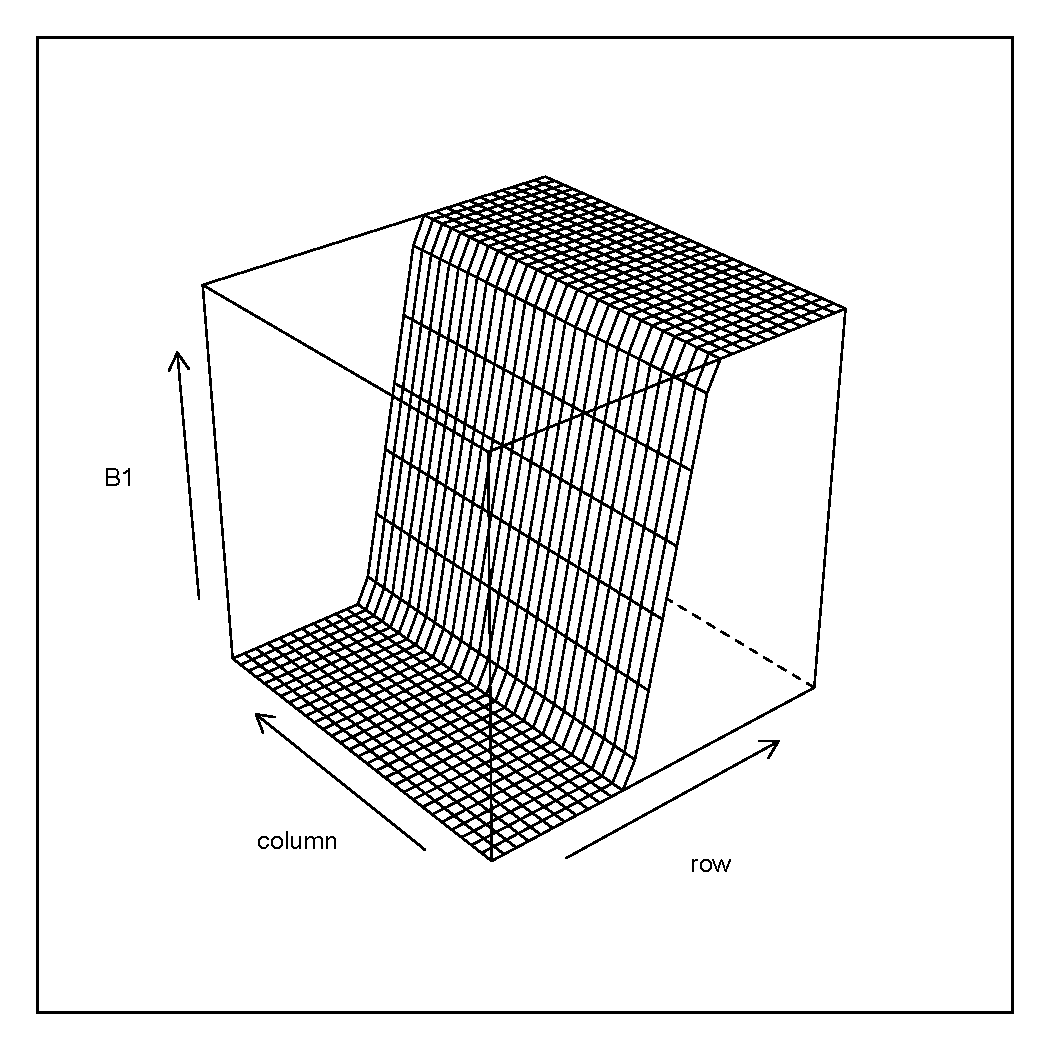
\includegraphics[width=0.33\textwidth]{0_Users_wesley_git_gwr_figures_simulation_step.pdf}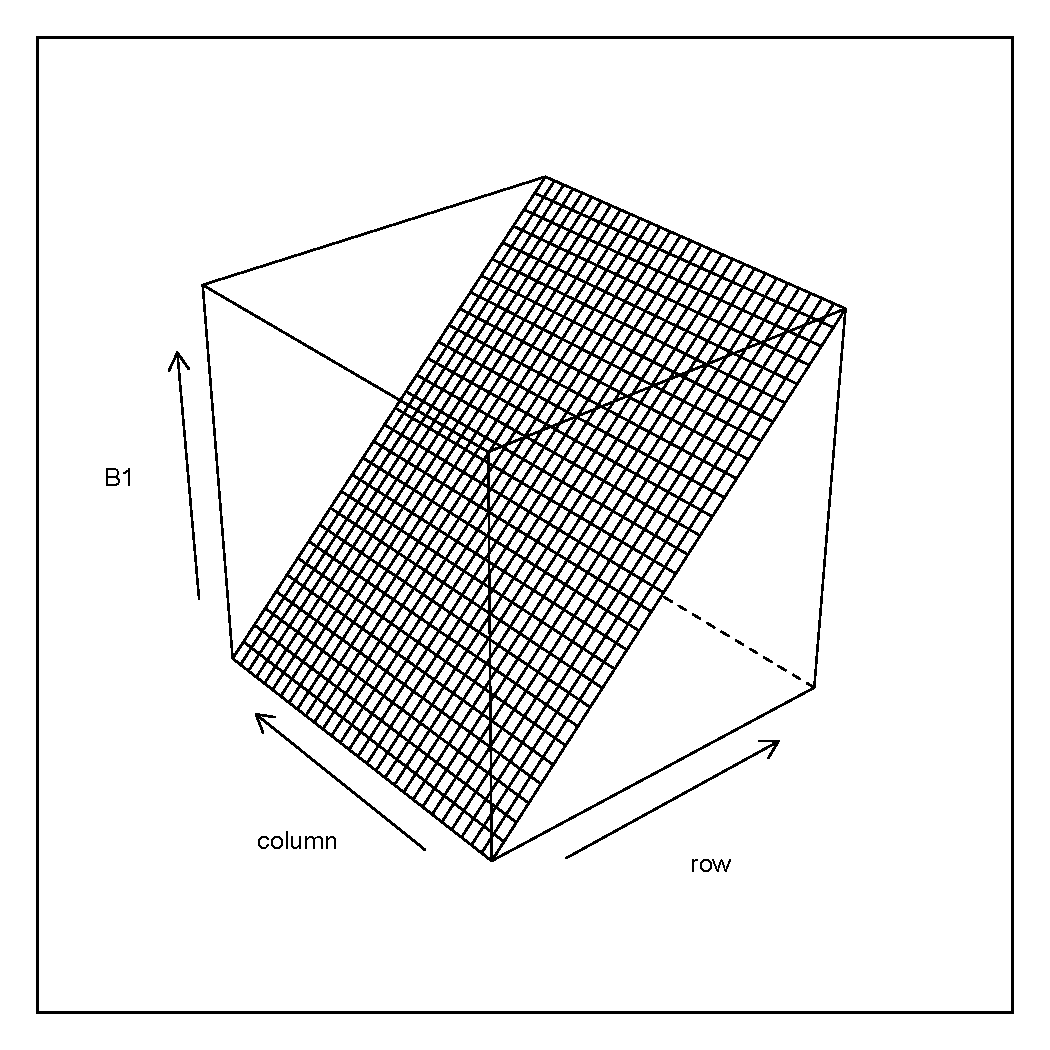
\includegraphics[width=0.33\textwidth]{1_Users_wesley_git_gwr_figures_simulation_gradient.pdf}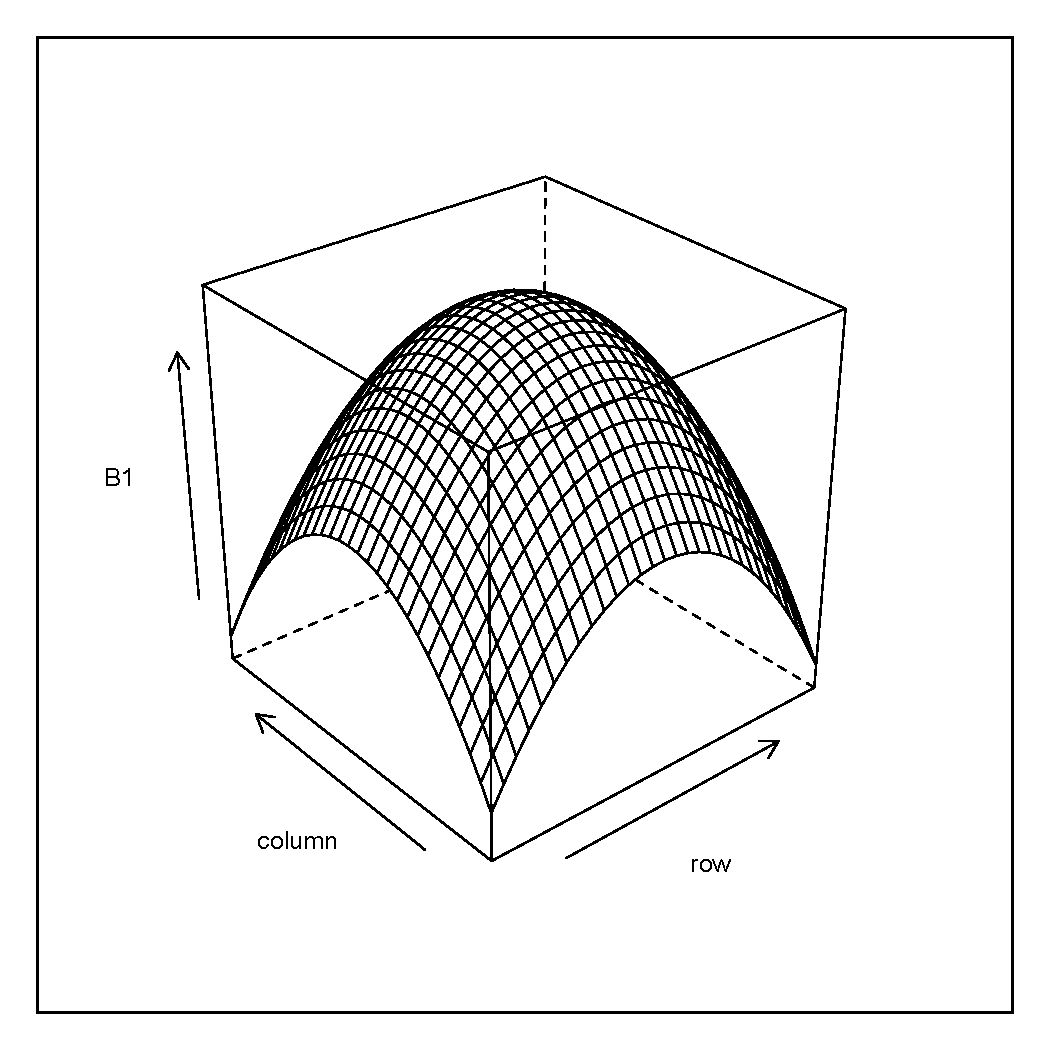
\includegraphics[width=0.33\textwidth]{2_Users_wesley_git_gwr_figures_simulation_parabola.pdf}

\protect\caption{These are, respectively, the step, gradient, and parabola functions
that were used for the coefficient function $\beta_{1}(\bm{s})$ in
the VCR model $y(\bm{s}_{i})=x_{1}(\bm{s}_{i})\beta_{1}(\bm{s}_{i})+\varepsilon(\bm{s}_{i})$
when generating the data for the simulation study.\label{fig:simulation-coefficient-functions}}
\end{figure}


In total, three parameters were varied to produce 18 settings, each
of which was simulated 100 times. There were the three functional
forms for the coefficient surface $\beta_{1}(\bm{s})$; data was simulated
both with low ($\rho=0$), medium ($\rho=0.5$), and high ($\rho=0.9$)
correlation between the covariates; and simulations were made with
low ($\sigma_{\varepsilon}=0.5$) and high ($\sigma_{\varepsilon}=1$)
variance for the random error term.



The results are presented in terms of the mean integrated squared
error (MISE) of the coefficient surface estimates $\hat{\beta}_{1}(\bm{s}),\dots,\hat{\beta}_{5}(\bm{s})$,
the MISE of the fitted response $\hat{y}(\bm{s})$, and the frequency
with which the coefficient surface estimates $\hat{\beta}_{2}(\bm{s}),\dots,\hat{\beta}_{5}(\bm{s})$
estimated by LAGR were zero. The performance of LAGR was compared
to that of a VCR model without variable selection, and to a VCR model
with oracular selection. Oracular selection means that exactly the
correct set of covariates was used to fit each local model.

\begin{table}
	\begin{tabular}{ccc|ccc|cc}
		\multicolumn{3}{c}{\begin{tabular}[c]{@{}c@{}}Simulation\\settings\end{tabular}} & \multicolumn{3}{c}{\begin{tabular}[c]{@{}c@{}}MISE\\$\hat{\beta}_1$\end{tabular}} & \multicolumn{2}{c}{\begin{tabular}[c]{@{}c@{}}MISE\\$\hat{\beta}_2, \dots, \hat{\beta}_5$\end{tabular}} \\
		$\beta_{1}(\bm{s})$ & $\rho$ & $\sigma_{\varepsilon}$ & LAGR & VCR & Oracle & LAGR & VCR \\
		\hline 

% latex table generated in R 3.1.0 by xtable 1.7-3 package
% Mon Jul 14 21:44:26 2014
  \multirow{6}{*}{step} & \multirow{2}{*}{0} & 0.5 & \emph{0.02} & 0.02 & \textbf{0.01} & \textbf{0.00} & 0.01 \\ 
    &  & 1.0 & \emph{0.03} & 0.03 & \textbf{0.02} & \textbf{0.00} & 0.02 \\ 
    & \multirow{2}{*}{0.5} & 0.5 & \emph{0.02} & 0.02 & \textbf{0.01} & \textbf{0.00} & 0.01 \\ 
    &  & 1.0 & \emph{0.03} & 0.05 & \textbf{0.02} & \textbf{0.00} & 0.03 \\ 
    & \multirow{2}{*}{0.9} & 0.5 & \emph{0.03} & 0.05 & \textbf{0.01} & \textbf{0.00} & 0.04 \\ 
    &  & 1.0 & \emph{0.12} & 0.17 & \textbf{0.02} & \textbf{0.02} & 0.15 \\ 
   \hline \multirow{6}{*}{gradient} & \multirow{2}{*}{0} & 0.5 & 0.01 & \emph{0.01} & \textbf{0.00} & \textbf{0.00} & 0.00 \\ 
    &  & 1.0 & 0.03 & \emph{0.02} & \textbf{0.01} & \textbf{0.00} & 0.02 \\ 
    & \multirow{2}{*}{0.5} & 0.5 & 0.01 & \emph{0.01} & \textbf{0.00} & \textbf{0.00} & 0.01 \\ 
    &  & 1.0 & 0.04 & \emph{0.03} & \textbf{0.01} & \textbf{0.00} & 0.03 \\ 
    & \multirow{2}{*}{0.9} & 0.5 & \emph{0.03} & 0.04 & \textbf{0.00} & \textbf{0.00} & 0.04 \\ 
    &  & 1.0 & \emph{0.14} & 0.14 & \textbf{0.01} & \textbf{0.02} & 0.15 \\ 
   \hline \multirow{6}{*}{parabola} & \multirow{2}{*}{0} & 0.5 & 0.01 & \emph{0.01} & \textbf{0.01} & \textbf{0.00} & 0.00 \\ 
    &  & 1.0 & 0.03 & \emph{0.02} & \textbf{0.02} & \textbf{0.00} & 0.02 \\ 
    & \multirow{2}{*}{0.5} & 0.5 & 0.01 & \emph{0.01} & \textbf{0.01} & \textbf{0.00} & 0.01 \\ 
    &  & 1.0 & 0.03 & \emph{0.03} & \textbf{0.02} & \textbf{0.00} & 0.03 \\ 
    & \multirow{2}{*}{0.9} & 0.5 & \emph{0.02} & 0.04 & \textbf{0.01} & \textbf{0.00} & 0.04 \\ 
    &  & 1.0 & 0.17 & \emph{0.14} & \textbf{0.02} & \textbf{0.03} & 0.15 \\ 
  

	\end{tabular}
	\caption{Listing of the simulation settings used to assess the performance of LAGR models versus oracle selection and no selection.}
	\label{tab:mise}
\end{table}


\subsection{Simulation Results}

The MISE of the estimates of $\beta_{1}(\bm{s})$ are in Table \ref{tab:misex}.
Recall that $\beta_{2}(\bm{s}),\dots,\beta_{5}(\bm{s})$ are exactly
zero across the entire domain. Oracle selection will estimate these
coefficients perfectly, so we focus on the comparison between estimation
by LAGR and by the VCR model with no selection. These results show
that for every simulation setting, LAGR estimation is more accurate
than the standard VCR model.



From Table \ref{tab:misey} we see that LAGR has good ability to identify
zero-coefficient covariates. The frequency with which $\beta_{2}(\bm{s}),\dots,\beta_{5}(\bm{s})$
were dropped from the LAGR models ranged from 0.78
to 0.97. The MISE of the fitted $\hat{y}(\bm{s})$
is listed in Table \ref{tab:misey}, where the highlighting is based
on which methods estimate an error variance that is closest to the
known truth for the simulation. The results are all very similar to
each other, indicating that no method was consistently better than
the others in this simulation at fitting the model output.

\begin{table}
	\begin{tabular}{ccc|c|ccc}
		\multicolumn{3}{c}{\begin{tabular}[c]{@{}c@{}}Simulation\\settings\end{tabular}} &  \multicolumn{1}{c}{\begin{tabular}[c]{@{}c@{}}Zero\\frequency\end{tabular}} &  \multicolumn{3}{c}{\begin{tabular}[c]{@{}c@{}}MISE\\$\hat{y}$\end{tabular}} \\
		$\beta_{1}(\bm{s})$ & $\rho$ & $\sigma_{\varepsilon}$ & $\hat{\beta}_2,\dots,\hat{\beta}_5 & LAGR & VCR & Oracle \\
		\hline 

% latex table generated in R 3.1.0 by xtable 1.7-3 package
% Mon Jul 14 21:44:29 2014
  \multirow{6}{*}{step} & \multirow{2}{*}{0} & 0.5 & 0.97 & \emph{0.25} & 0.26 & \textbf{0.25} \\ 
    &  & 1.0 & 0.96 & \emph{1.00} & \textbf{1.00} & 0.99 \\ 
    & \multirow{2}{*}{0.5} & 0.5 & 0.96 & \emph{0.26} & 0.26 & \textbf{0.25} \\ 
    &  & 1.0 & 0.92 & \emph{0.99} & \textbf{1.00} & 0.98 \\ 
    & \multirow{2}{*}{0.9} & 0.5 & 0.86 & \emph{0.27} & 0.30 & \textbf{0.25} \\ 
    &  & 1.0 & 0.85 & \emph{1.08} & 1.14 & \textbf{0.98} \\ 
   \hline \multirow{6}{*}{gradient} & \multirow{2}{*}{0} & 0.5 & 0.96 & \emph{0.25} & \textbf{0.25} & 0.25 \\ 
    &  & 1.0 & 0.95 & \textbf{0.99} & \emph{0.99} & 0.97 \\ 
    & \multirow{2}{*}{0.5} & 0.5 & 0.94 & \emph{0.25} & \textbf{0.25} & 0.24 \\ 
    &  & 1.0 & 0.92 & \emph{1.00} & \textbf{1.00} & 0.97 \\ 
    & \multirow{2}{*}{0.9} & 0.5 & 0.80 & \emph{0.27} & 0.28 & \textbf{0.24} \\ 
    &  & 1.0 & 0.85 & \emph{1.09} & 1.12 & \textbf{0.97} \\ 
   \hline \multirow{6}{*}{parabola} & \multirow{2}{*}{0} & 0.5 & 0.97 & \emph{0.25} & \textbf{0.25} & 0.25 \\ 
    &  & 1.0 & 0.94 & \textbf{1.00} & \emph{1.00} & 0.98 \\ 
    & \multirow{2}{*}{0.5} & 0.5 & 0.95 & \textbf{0.25} & 0.25 & \emph{0.25} \\ 
    &  & 1.0 & 0.88 & \textbf{1.00} & \emph{1.00} & 0.97 \\ 
    & \multirow{2}{*}{0.9} & 0.5 & 0.79 & \emph{0.26} & 0.28 & \textbf{0.24} \\ 
    &  & 1.0 & 0.78 & 1.13 & \emph{1.12} & \textbf{0.98} \\ 
  
	\end{tabular}
	\caption{The MISE for the fitted output in each simulation setting, under variable selection via LAGR, no variable selection, and oracular variable selection. Highlighting indicates the \textbf{closest} and \emph{next-closest} to the actual error variance $\sigma_\varepsilon^2$ for that setting.}
	\label{tab:misey}
\end{table}

The proposed LAGR method was accurate in selection and estimation,
with estimation accuracy for $\beta_{1}(\bm{s})$ about equal to that
of the VCR model with no selection, and with consistently better accuracy
for estimating $\beta_{2}(\bm{s}),\dots,\beta_{5}(\bm{s})$.

There was minimal difference in the performance of the proposed LAGR
method between low ($\sigma_{\varepsilon}=0.5$) and high ($\sigma_{\varepsilon}=1$)
error variance, and between no ($\rho=0$) and moderate ($\rho=0.5$)
correlation among the covariates. But the selection and estimation
accuracy did decline when there was high ($\rho=0.9$) correlation
among the predictor variables.


\section{Data Example\label{sec:example}}




The proposed LAGR estimation method was used to estimate the coefficients
in a VCR model of the effect of some covariates on the price of homes
in Boston \citep{Harrison-Rubinfeld-1978,Gilley-Pace-1996,Pace-Gilley-1997}.
The data source is based on the 1970 U.S. census. In the data, we
have the median price of homes sold in 506 census tracts (MEDV), along
with some potential covariates. The covariates are CRIM (the per-capita
crime rate in the tract), RM (the mean number of rooms for houses
sold in the tract), RAD (an index of how accessible the tract is from
Boston's radial roads), TAX (the property tax per \$10,000 of property
value), and LSTAT (the percentage of the tract's residents who are
considered ``lower status''). The bandwidth parameter was set to
0.2 for a nearest neighbors-type bandwidth, meaning that the sum of
kernel weights for each local model was 20\% of the total number of
observations. The kernel used was the Epanechnikov kernel.

A summary of the local coefficients is in Table \ref{tab:boston-coefs-lagr}.
It indicates that RM is the only predictor variable with a positive
mean of the local coefficients. The coefficient of the CRIM variable
was estimated to be exactly zero at 49\%
of the locations. The percentage for the RAD variable was 37\%.

\begin{figure}

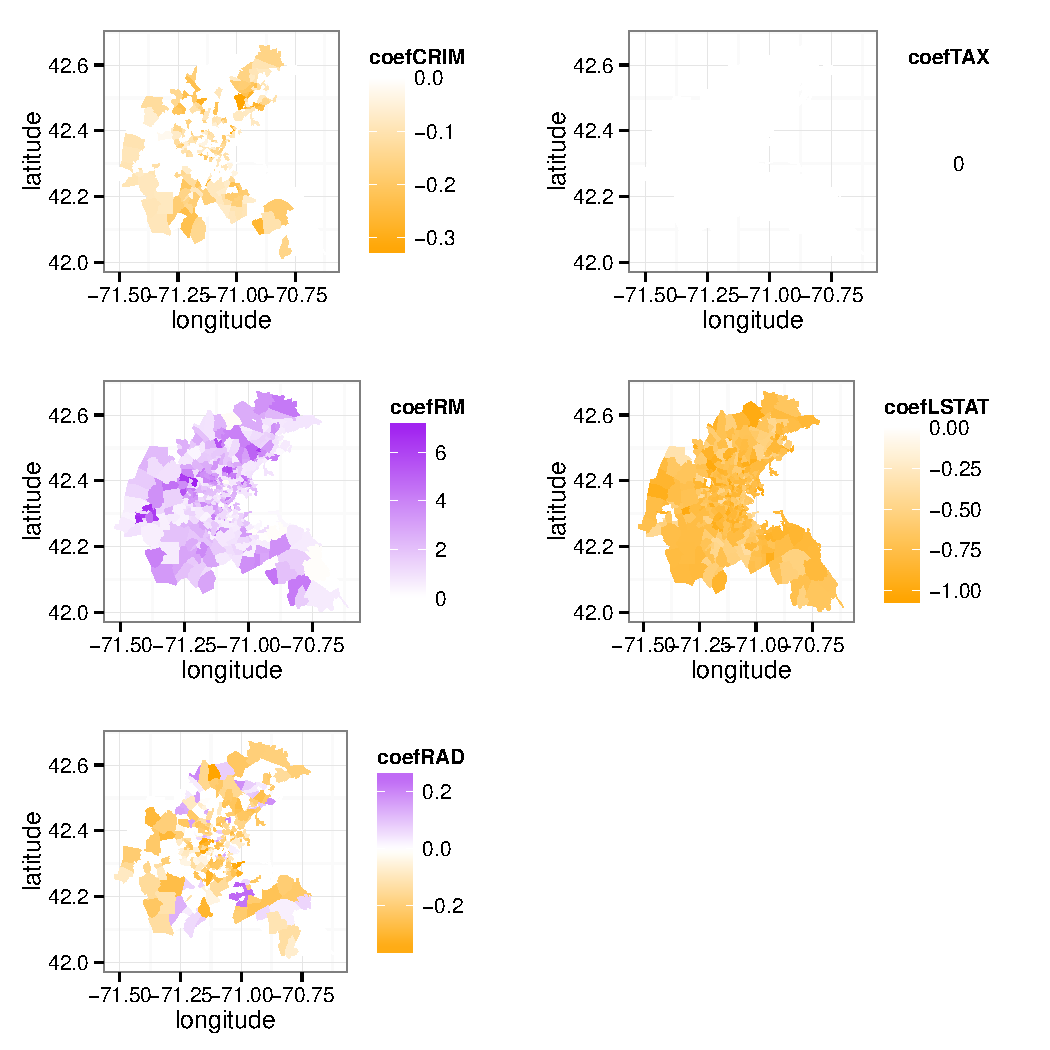
\includegraphics[width=\maxwidth]{figure/boston-plots} 


\caption{The LAGR estimates of coefficients for the Boston house price data.\label{fig:boston-lagr-coefs}}
\end{figure}

Estimates of the regression coefficients are plotted in Figure \ref{fig:boston-lagr-coefs}.
One interesting result is that LAGR indicates that the TAX variable
was nowhere an important predictor of the median house price. Another
is that the coefficients of CRIM and LSTAT are everywhere negative
or zero (meaning that a greater crime rate or proportion of lower-status
individuals is associated with a lower median house price where the
effect is discernable) and that of RM is positive (meaning that a
greater average number of rooms per house is associated with a greater
median house price). The coefficient of RAD is positive in some areas
and negative in others. This indicates that there are parts of Boston
where improved access to radial roads is associates with a greater
median house price and parts where it is associated with a lesser
median house price.

% latex table generated in R 3.1.0 by xtable 1.7-3 package
% Mon Jul 14 21:44:35 2014
\begin{table}
\centering
\begin{tabular}{rrrr}
  & Mean & SD & Prop. zero \\ 
  \hline
CRIM & -0.07 & 0.08 & 0.49 \\ 
  RM & 1.92 & 1.43 & 0.02 \\ 
  RAD & -0.08 & 0.13 & 0.37 \\ 
  TAX & 0.00 & 0.00 & 1.00 \\ 
  LSTAT & -0.72 & 0.16 & 0.01 \\ 
  \end{tabular}
\caption{The mean, standard deviation, and proportion of zeros among the local coefficients in a model for the median house price in census tracts in Boston, with coefficients selected and fitted by LAGR.} 
\label{tab:boston-coefs-lagr}
\end{table}


In their example using the same data, \citet{Sun-Yan-Zhang-Lu-2014}
estimated that the coefficients of RAD annd LSTAT should be constant,
at $0.36$ and $-0.45$, respectively. That conclusion differs from
our result, which says that the mean local coefficient of RAD is actually
negative (\ensuremath{-0.08}), while
our mean fitted local coefficient for LSTAT was more negative than
the estimate of \citet{Sun-Yan-Zhang-Lu-2014}.


\section{Extension to GLMs\label{sec:lagr-gllm}}


\subsection{Model}

Generalized linear models (GLM) extend the linear model to distributions
other than gaussian. The generalized local linear model (GLLM) is
an extension of the GLM to varying coefficient models via local regression.

As was the case for local linear regression models, the GLLM coefficients
are smooth functions of location, called $\bm{\beta}(\bm{s})$. If
the response variable $y$ is from an exponential-family distribution
then its density is 

\[
f\left(y\left(\bm{s}\right)|\bm{x}\left(\bm{s}\right),\theta\left(\bm{s}\right)\right)=c\left(y\left(\bm{s}\right)\right)\times\exp\left[\theta\left(\bm{s}\right)y\left(\bm{s}\right)-b\left(\theta\left(\bm{s}\right)\right)\right]
\]


where $\phi$ and $\theta$ are parameters and

\begin{align*}
E\left\{ y(\bm{s})|\bm{x}(\bm{s})\right\} = & \mu(\bm{s})=b'\left(\theta\left(\bm{s}\right)\right)\\
\theta\left(\bm{s}\right)= & (g\circ b')^{-1}\left(\eta\left(\bm{s}\right)\right)\\
\eta\left(\bm{s}\right)= & \bm{x}^{T}\left(\bm{s}\right)\bm{\beta}\left(\bm{s}\right)=g\left(\mu\left(\bm{s}\right)\right)\\
\text{\text{Var}}\left\{ y\left(\bm{s}\right)|\bm{x}\left(\bm{s}\right)\right\} = & b''\left(\theta\left(\bm{s}\right)\right)
\end{align*}


The function $g(\cdot)$ is called the link function. If its inverse
$g^{-1}(\cdot)=b'(\cdot)$ then the composition $\left(g\circ b'\right)\left(\cdot\right)$
is the identity function. This particular choice of $g$ is called
the canonical link. We follow the practice of \citet{Fan-Heckman-Wand-1995}
in assuming the use of the canonical link.

Under the canonical link function, the expressions for the mean and
variance of the response variable can be simplified to

\begin{align*}
E\left\{ y(\bm{s})|\bm{x}(\bm{s})\right\} = & g^{-1}\left(\eta(\bm{s})\right)\\
\text{\text{Var}}\left\{ y(\bm{s})|\bm{x}(\bm{s})\right\} = & \left[g'\left(\mu(\bm{s})\right)\right]^{-1}=V\left(\mu(\bm{s})\right)\\
\frac{d}{d\mu} & g^{-1}\left(\mu\left(\bm{s}\right)\right)=V\left(\mu\left(\bm{s}\right)\right)
\end{align*}
 


\subsection{Local quasi-likelihood}

Assuming the canonical link, all that is required is to specify the
mean-variance relationship via the variance function, $V\left\{ \mu(\bm{s})\right\} $.
Then the GLLM coefficients can be estimated by maximizing the local
quasi-likelihood 

\begin{align}
\mathcal{\ell}^{*}\left(\bm{\zeta}(\bm{s})\right) & =\sum_{i=1}^{n}K_{h}\left(\|\bm{s}-\bm{s}_{i}\|\right)Q\left(g^{-1}\left(\bm{z}'(\bm{s}_{i})\bm{\zeta}(\bm{s})\right),Y(\bm{s}_{i})\right).
\end{align}


The local quasi-likelihood generalizes the local log-likelihood that
was used to estimate coefficients in the local linear model case.
The quasi-likelihood is convex, and is defined in terms of its derivative,
the quasi-score function

\[
\frac{\partial}{\partial\mu}Q\left(\mu,y\right)=\frac{y-\mu}{V\left(\mu\right)}.
\]



\subsection{Estimation}

Under these conditions, the local quasi-likelihood is maximized where

\begin{align}
\frac{\partial}{\partial\bm{\zeta}}\mathcal{\ell}^{*}\left(\hat{\bm{\zeta}}\left(\bm{s}\right)\right) & =\sum_{i=1}^{n}K_{h}\left(\|\bm{s}-\bm{s}_{i}\|\right)\frac{y\left(\bm{s}_{i}\right)-\hat{\mu}\left(\bm{s}_{i};\bm{s}\right)}{V\left(\hat{\mu}\left(\bm{s}_{i};\bm{s}\right)\right)}\bm{z}\left(\bm{s}_{i}\right)=\bm{0}_{3p}
\end{align}


and $\hat{\mu}\left(\bm{s}_{i};\bm{s}\right)=g^{-1}\left(\bm{z}'\left(\bm{s}_{i}\right)\hat{\bm{\zeta}}\left(\bm{s}\right)\right)$
is the mean at location $\bm{s}_{i}$ estimated using the coefficients
$\hat{\bm{\zeta}}\left(\bm{s}\right)$ fitted at location $\bm{s}$.
Except for the $K_{h}\left(\|\bm{s}-\bm{s}_{i}\|\right)$ term, this
is the same as the normal equations for estimating coefficients in
a GLM. The method of iteratively reweighted least squares (IRLS) is
used to solve for $\hat{\bm{\zeta}}\left(\bm{s}\right)$.


\subsection{Distribution of the local coefficients}

The asymptotic distribution of the local coefficients in a varying-coefficients
GLM with a one-dimensional effect-modifying parameter are given in
\citet{Cai-Fan-Li-2000}. For coefficients that vary in two dimensions
(e.g. spatial location), the asymptotic distribution under the canonical
link is

\[
\sqrt{{nh^{2}f(\bm{{s}})}}\left[\hat{\bm{\beta}}(\bm{s})-\bm{\beta}(\bm{s})-(1/2)\kappa_{0}^{-1}\kappa_{2}h^{2}\left\{ \bm{\beta}_{uu}(\bm{s})+\bm{\beta}_{vv}(\bm{s})\right\} \right]\xrightarrow{{D}}N\left(\bm{0},\kappa_{0}^{-2}\nu_{0}\Gamma^{-1}(\bm{s})\right)
\]


where $\Gamma(\bm{s})=E\left[V\left(\mu(\bm{s})\right)X(\bm{s})X(\bm{s})^{T}\right]$.


\subsection{LAGR penalty}

As in the case of linear models, the LAGR for GLMs is a grouped $\ell_{1}$
regularization method. Now, though, we use a penalized local quasi-likelihood:

\begin{align}
\mathcal{J}\left(\bm{\zeta}(\bm{s})\right) & =\mathcal{\ell}^{*}\left(\bm{\zeta}(\bm{s})\right)+\mathcal{P}\left(\bm{\zeta}(\bm{s})\right)\label{eq:adaptive-lasso-GLLM}\\
 & =\sum_{i=1}^{n}K_{h}\left(\|\bm{s}-\bm{s}_{i}\|\right)Q\left(g^{-1}\left(z'(\bm{s}_{i})\bm{\zeta}(\bm{s})\right),Y(\bm{s}_{i})\right)+\sum_{j=1}^{p}\phi_{j}\left(\bm{s}\right)\|\bm{\zeta}_{j}\left(\bm{s}\right)\|
\end{align}


and similarly to the case for gaussian data, $\phi_{j}\left(\bm{s}\right)=\lambda_{n}\left(\bm{s}\right)\|\tilde{\bm{\zeta}}_{j}\left(\bm{s}\right)\|^{-\gamma}$,
where $\lambda_{n}\left(\bm{s}\right)>0$ is a the local tuning parameter
applied to all coefficients at location $\bm{s}$ and $\tilde{\bm{\zeta}}_{j}\left(\bm{s}\right)$
is the vector of unpenalized local coefficients.


\subsection{Oracle properties of LAGR in the GLM setting}

The oracle properties for LAGR in the GLM setting are similar to those
in the gaussian setting:
\begin{thm}[Asymptotic normality]
\label{theorem:normality-glm} 



If $h^{-1}n^{-1/2}a_{n}\xrightarrow{p}0$ and $hn^{-1/2}b_{n}\xrightarrow{p}\infty$
then 
\[
h\sqrt{n}\left[\hat{\bm{\beta}}_{a}(\bm{s})-\bm{\beta}_{a}(\bm{s})-\frac{\kappa_{2}h^{2}}{2\kappa_{0}}\left\{ \nabla_{uu}^{2}\bm{\beta}_{a}(\bm{s})+\nabla_{vv}^{2}\bm{\beta}_{a}(\bm{s})\right\} \right]\xrightarrow{d}N\left(0,f\left(\bm{s}\right)^{-1}\kappa_{0}^{-2}\nu_{0}\Gamma^{-1}(\bm{s})\right)
\]

\end{thm}

\begin{thm}[Selection consistency]
\label{theorem:selection-glm}



If $h^{-1}n^{-1/2}a_{n}\xrightarrow{p}\infty$ and $hn^{-1/2}b_{n}\xrightarrow{p}\infty$
then $Pr\left\{ \|\hat{\bm{\zeta}}_{j}(\bm{s})\|=\utilde{0}\right\} \to0$
if $j\le p_{0}$ and $Pr\left\{ \|\hat{\bm{\zeta}}_{j}(\bm{s})\|=\utilde{0}\right\} \to1$
if $j>p_{0}$. 
\end{thm}
\appendix

\section*{Appendix: Proofs of Theorem \ref{theorem:normality}\label{sec:gaussian-normality-proof} }
\begin{proof}
Let $H_{n}(\bm{u})=\mathcal{J}\left(\bm{\zeta}\left(\bm{s}\right)+h^{-1}n^{-1/2}\bm{u}\right)-\mathcal{J}\left(\bm{\zeta}\left(\bm{s}\right)\right)$.
Then, we have 
\begin{align}
H_{n}\left(\bm{u}\right)= & (1/2)\left[\bm{Y}-\bm{Z}(\bm{s})\left\{ \bm{\zeta}\left(\bm{s}\right)+h^{-1}n^{-1/2}\bm{u}\right\} \right]^{T}\bm{W}(\bm{s})\left[\bm{Y}-\bm{Z}(\bm{s})\left\{ \bm{\zeta}\left(\bm{s}\right)+h^{-1}n^{-1/2}\bm{u}\right\} \right]\\
 & +\sum_{j=1}^{p}\phi_{j}(\bm{s})\|\bm{\zeta}_{j}(\bm{s})+h^{-1}n^{-1/2}\bm{u}_{j}\|\\
 & -(1/2)\left\{ \bm{Y}-\bm{Z}(\bm{s})\bm{\zeta}(\bm{s})\right\} ^{T}\bm{W}(\bm{s})\left\{ \bm{Y}-\bm{Z}(\bm{s})\bm{\zeta}(\bm{s})\right\} -\sum_{j=1}^{p}\phi_{j}(\bm{s})\|\bm{\zeta}_{j}(\bm{s})\|\\
= & (1/2)\bm{u}^{T}\left\{ h^{-2}n^{-1}\bm{Z}^{T}(\bm{s})\bm{W}(\bm{s})\bm{Z}(\bm{s})\right\} \bm{u}\\
 & -\bm{u}^{T}\left[h^{-1}n^{-1/2}\bm{Z}^{T}(\bm{s})\bm{W}(\bm{s})\left\{ \bm{Y}-\bm{Z}(\bm{s})\bm{\zeta}(\bm{s})\right\} \right]\\
 & +\sum_{j=1}^{p}n^{-1/2}\phi_{j}(\bm{s})n^{1/2}\left\{ \|\bm{\zeta}_{j}(\bm{s})+h^{-1}n^{-1/2}\bm{u}_{j}\|-\|\bm{\zeta}_{j}(\bm{s})\|\right\} 
\end{align}


Note that the limiting behavior of the last term differs between the
cases $j\le p_{0}$ and $j>p_{0}$.

Case $j\le p_{0}$:

If $j\le p_{0}$, then $n^{-1/2}\phi_{j}(\bm{s})\to n^{-1/2}\lambda_{n}(\bm{s})\|\bm{\zeta}_{j}(\bm{s})\|^{-\gamma}$
and $|\sqrt{n}\left\{ \|\bm{\zeta}_{j}(\bm{s})+h^{-1}n^{-1/2}\bm{u}_{j}\|-\|\bm{\zeta}_{j}(\bm{s})\|\right\} |\le h^{-1}\|\bm{u}_{j}\|$
. Thus, 
\[
\lim\limits _{n\to\infty}\phi_{j}(\bm{s})\left(\|\bm{\zeta}_{j}(\bm{s})+h^{-1}n^{-1/2}\bm{u}_{j}\|-\|\bm{\zeta}_{j}(\bm{s})\|\right)\le h^{-1}n^{-1/2}\phi_{j}(\bm{s})\|\bm{u}_{j}\|\le h^{-1}n^{-1/2}a_{n}\|\bm{u}_{j}\|\to0
\]


Case $j>p_{0}$:

If $j>p_{0}$, then $\phi_{j}(\bm{s})\left(\|\bm{\zeta}_{j}(\bm{s})+h^{-1}n^{-1/2}\bm{u}_{j}\|-\|\bm{\zeta}_{j}(\bm{s})\|\right)=\phi_{j}(\bm{s})h^{-1}n^{-1/2}\|\bm{u}_{j}\|$.

Since $h=O(n^{-1/6})$, if $hn^{-1/2}b_{n}\xrightarrow{p}\infty$,
then $h^{-1}n^{-1/2}b_{n}\xrightarrow{p}\infty$.

Now, if $\|\bm{u}_{j}\|\ne0$, then 
\[
h^{-1}n^{-1/2}\phi_{j}(\bm{s})\|\bm{u}_{j}\|\ge h^{-1}n^{-1/2}b_{n}\|\bm{u}_{j}\|\to\infty.
\]
On the other hand, if $\|\bm{u}_{j}\|=0$, then $h^{-1}n^{-1/2}\phi_{j}(\bm{s})\|\bm{u}_{j}\|=0$.

Thus, the limit of $H_{n}\left(\bm{u}\right)$ is the same as the
limit of $H_{n}^{*}\left(\bm{u}\right)$ where

\[
H_{n}^{*}\left(\bm{u}\right)=(1/2)\bm{u}^{T}\left\{ h^{-2}n^{-1}\bm{Z}^{T}(\bm{s})\bm{W}(\bm{s})\bm{Z}(\bm{s})\right\} \bm{u}-\bm{u}^{T}\left[h^{-1}n^{-1/2}\bm{Z}^{T}(\bm{s})\bm{W}(\bm{s})\left\{ \bm{Y}-\bm{Z}(\bm{s})\bm{\zeta}(\bm{s})\right\} \right]
\]


if $\|\bm{u}_{j}\|=0\;\forall j>p_{0}$, and $H_{n}^{*}\left(\bm{u}\right)=\infty$
otherwise. It follows that $H_{n}^{*}\left(\bm{u}\right)$ is convex
and its unique minimizer $\hat{\bm{u}}_{n}$ is found by solving the
equation:

\begin{align}
\utilde{0} & =\left\{ h^{-2}n^{-1}\bm{Z}\left(\bm{s}\right)^{T}\bm{W}\left(\bm{s}\right)\bm{Z}\left(\bm{s}\right)\right\} \hat{\bm{u}}_{n}-\left[h^{-1}n^{-1/2}\bm{Z}\left(\bm{s}\right)^{T}\bm{W}\left(\bm{s}\right)\left\{ \bm{Y}-\bm{Z}\left(\bm{s}\right)\bm{\zeta}\left(\bm{s}\right)\right\} \right].\label{eq:limit}
\end{align}


That is, $\hat{\bm{u}}_{n}=\left\{ n^{-1}\bm{Z}^{T}\left(\bm{s}\right)\bm{W}\left(\bm{s}\right)\bm{Z}\left(\bm{s}\right)\right\} ^{-1}\left[hn^{-1/2}\bm{Z}\left(\bm{s}\right)^{T}\bm{W}\left(\bm{s}\right)\left\{ \bm{Y}-\bm{Z}\left(\bm{s}\right)\bm{\zeta}\left(\bm{s}\right)\right\} \right]$.

By epiconvergence results, the minimizer of the limiting function
is the limit of the minimizers $\hat{\bm{u}}^{(n)}$ \citep{Geyer-1994,Knight-Fu-2000}.
Since, by Lemma 2 of \citet{Sun-Yan-Zhang-Lu-2014},

\begin{equation}
\hat{\bm{u}}_{n}\xrightarrow{d}N\left(\frac{\kappa_{2}h^{2}}{2\kappa_{0}}\{\nabla_{uu}^{2}\bm{\zeta}_{j}(\bm{s})+\nabla_{vv}^{2}\bm{\zeta}_{j}(\bm{s})\},f(\bm{s})\kappa_{0}^{-2}\nu_{0}\sigma^{2}\Psi^{-1}\right)
\end{equation}
the result of Theorem \ref{theorem:normality} follows.
\end{proof}

\section*{Appendix: Proof of Theorem \ref{theorem:selection}\label{sec:gaussian-selection-proof}}
\begin{proof}
We showed in Theorem \ref{theorem:normality} that $\hat{\bm{\zeta}}_{j}\left(\bm{s}\right)\xrightarrow{p}\bm{\zeta}_{j}\left(\bm{s}\right)+\frac{\kappa_{2}h^{2}}{2\kappa_{0}}\{\nabla_{uu}^{2}\bm{\zeta}_{j}\left(\bm{s}\right)+\nabla_{vv}^{2}\bm{\zeta}_{j}\left(\bm{s}\right)\}$,
so to complete the proof of selection consistency, it only remains
to show that $Pr\left\{ \hat{\bm{\zeta}}_{j}\left(\bm{s}\right)=\utilde{0}\right\} \to1$
if $j>p_{0}$.

The proof is by contradiction. Without loss of generality we consider
only the case $j=p$.

Assume $\|\hat{\bm{\zeta}}_{p}(\bm{s})\|\ne0$. Then $\mathcal{J}\left(\bm{\zeta}\left(\bm{s}\right)\right)$
is differentiable w.r.t. $\bm{\zeta}_{p}\left(\bm{s}\right)$ and
is minimized where 
\begin{align}
\utilde{0}= & \bm{Z}_{p}^{T}\left(\bm{s}\right)\bm{W}\left(\bm{s}\right)\left\{ \bm{Y}-\bm{Z}_{-p}\left(\bm{s}\right)\hat{\bm{\zeta}}_{-p}\left(\bm{s}\right)-\bm{Z}_{p}\left(\bm{s}\right)\hat{\bm{\zeta}}_{p}\left(\bm{s}\right)\right\} -\phi_{p}(\bm{s})\frac{\hat{\bm{\zeta}}_{p}\left(\bm{s}\right)}{\|\hat{\bm{\zeta}}_{p}\left(\bm{s}\right)\|}\\
= & \bm{Z}_{p}\left(\bm{s}\right)^{T}\bm{W}\left(\bm{s}\right)\left[\bm{Y}-\bm{Z}\left(\bm{s}\right)\bm{\zeta}\left(\bm{s}\right)-\frac{h^{2}\kappa_{2}}{2\kappa_{0}}\left\{ \nabla_{uu}^{2}\bm{\zeta}\left(\bm{s}\right)+\nabla_{vv}^{2}\bm{\zeta}\left(\bm{s}\right)\right\} \right]\\
 & +\bm{Z}_{p}\left(\bm{s}\right)^{T}\bm{W}\left(\bm{s}\right)\bm{Z}_{-p}\left(\bm{s}\right)\left[\bm{\zeta}_{-p}\left(\bm{s}\right)+\frac{h^{2}\kappa_{2}}{2\kappa_{0}}\left\{ \nabla_{uu}^{2}\bm{\zeta}_{-p}\left(\bm{s}\right)+\nabla_{vv}^{2}\bm{\zeta}_{-p}\left(\bm{s}\right)\right\} -\hat{\bm{\zeta}}_{-p}\left(\bm{s}\right)\right]\\
 & +\bm{Z}_{p}\left(\bm{s}\right)^{T}\bm{W}\left(\bm{s}\right)\bm{Z}_{p}\left(\bm{s}\right)\left[\bm{\zeta}_{p}\left(\bm{s}\right)+\frac{h^{2}\kappa_{2}}{2\kappa_{0}}\left\{ \nabla_{uu}^{2}\bm{\zeta}_{p}\left(\bm{s}\right)+\nabla_{vv}^{2}\bm{\zeta}_{p}\left(\bm{s}\right)\right\} -\hat{\bm{\zeta}}_{p}\left(\bm{s}\right)\right]\\
 & -\phi_{p}\left(\bm{s}\right)\frac{\hat{\bm{\zeta}}_{p}\left(\bm{s}\right)}{\|\hat{\bm{\zeta}}_{p}\left(\bm{s}\right)\|}
\end{align}


Thus, 
\begin{align}
\frac{h}{\sqrt{n}}\phi_{p}\left(\bm{s}\right)\frac{\hat{\bm{\zeta}}_{p}\left(\bm{s}\right)}{\|\hat{\bm{\zeta}}_{p}\left(\bm{s}\right)\|}=\label{eq:selection}\\
 & \bm{Z}_{p}\left(\bm{s}\right)^{T}\bm{W}\left(\bm{s}\right)\frac{h}{\sqrt{n}}\left[\bm{Y}-\bm{Z}\left(\bm{s}\right)\bm{\zeta}\left(\bm{s}\right)-\frac{h^{2}\kappa_{2}}{2\kappa_{0}}\left\{ \nabla_{uu}^{2}\bm{\zeta}\left(\bm{s}\right)+\nabla_{vv}^{2}\bm{\zeta}\left(\bm{s}\right)\right\} \right]\\
 & +\left\{ n^{-1}\bm{Z}_{p}\left(\bm{s}\right)^{T}\bm{W}(\bm{s})\bm{Z}_{-p}\left(\bm{s}\right)\right\} h\sqrt{n}\left[\bm{\zeta}_{-p}\left(\bm{s}\right)+\frac{h^{2}\kappa_{2}}{2\kappa_{0}}\left\{ \nabla_{uu}^{2}\bm{\zeta}_{-p}\left(\bm{s}\right)+\nabla_{vv}^{2}\bm{\zeta}_{-p}\left(\bm{s}\right)\right\} -\hat{\bm{\zeta}}_{-p}\left(\bm{s}\right)\right]\notag\\
 & +\left\{ n^{-1}\bm{Z}_{p}\left(\bm{s}\right)^{T}\bm{W}\left(\bm{s}\right)\bm{Z}_{p}\left(\bm{s}\right)\right\} h\sqrt{n}\left[\bm{\zeta}_{p}\left(\bm{s}\right)+\frac{h^{2}\kappa_{2}}{2\kappa_{0}}\left\{ \nabla_{uu}^{2}\bm{\zeta}_{p}\left(\bm{s}\right)+\nabla_{vv}^{2}\bm{\zeta}_{p}\left(\bm{s}\right)\right\} -\hat{\bm{\zeta}}_{p}\left(\bm{s}\right)\right]
\end{align}


From Lemma 2 of \citet{Sun-Yan-Zhang-Lu-2014}, $\left\{ n^{-1}\bm{Z}_{p}\left(\bm{s}\right)^{T}\bm{W}\left(\bm{s}\right)\bm{Z}_{-p}\left(\bm{s}\right)\right\} =O_{p}\left(1\right)$
and $\left\{ n^{-1}\bm{Z}_{p}\left(\bm{s}\right)^{T}\bm{W}\left(\bm{s}\right)\bm{Z}_{p}\left(\bm{s}\right)\right\} =O_{p}\left(1\right)$.

From Theorem 3 of \citet{Sun-Yan-Zhang-Lu-2014}, we have that $h\sqrt{n}\left[\hat{\bm{\zeta}}_{-p}\left(\bm{s}\right)-\bm{\zeta}_{-p}\left(\bm{s}\right)-\frac{h^{2}\kappa_{2}}{2\kappa_{0}}\left\{ \nabla_{uu}^{2}\zeta_{-p}\left(\bm{s}\right)+\nabla_{vv}^{2}\zeta_{-p}\left(\bm{s}\right)\right\} \right]=O_{p}\left(1\right)$
and $h\sqrt{n}\left[\hat{\bm{\zeta}}_{p}\left(\bm{s}\right)-\bm{\zeta}_{p}\left(\bm{s}\right)-\frac{h^{2}\kappa_{2}}{2\kappa_{0}}\left\{ \nabla_{uu}^{2}\zeta_{p}\left(\bm{s}\right)+\nabla_{vv}^{2}\zeta_{p}\left(\bm{s}\right)\right\} \right]=O_{p}\left(1\right)$.

We showed in the proof of Theorem \ref{theorem:normality} that

\[
h\sqrt{n}\bm{Z}_{p}\left(\bm{s}\right)^{T}\bm{W}\left(\bm{s}\right)\left[\bm{Y}-\bm{Z}\left(\bm{s}\right)\bm{\zeta}\left(\bm{s}\right)-\frac{h^{2}\kappa_{2}}{2\kappa_{0}}\left\{ \nabla_{uu}^{2}\bm{\zeta}\left(\bm{s}\right)+\nabla_{vv}^{2}\bm{\zeta}\left(\bm{s}\right)\right\} \right]=O_{p}\left(1\right).
\]


The right hand side of (\ref{eq:selection}) is $O_{p}(1)$, so for
$\hat{\bm{\zeta}}_{p}\left(\bm{s}\right)$ to be a solution, we must
have that $hn^{-1/2}\phi_{p}\left(\bm{s}\right)\hat{\bm{\zeta}}_{p}\left(\bm{s}\right)/\|\hat{\bm{\zeta}}_{p}\left(\bm{s}\right)\|=O_{p}\left(1\right)$.

But since by assumption $\hat{\bm{\zeta}}_{p}\left(\bm{s}\right)\ne\utilde{0}$,
there must be some $k\in\{1,2,3\}$ such that $|\hat{\zeta}_{p_{k}}\left(\bm{s}\right)|=\max\{|\hat{\zeta}_{p_{k'}}\left(\bm{s}\right)|:1\le k'\le3\}$.
And for this $k$, we have that $|\hat{\zeta}_{p_{k}}\left(\bm{s}\right)|/\|\hat{\bm{\zeta}}_{p}\left(\bm{s}\right)\|\ge1/\sqrt{3}>0$.

Since $hn^{-1/2}b_{n}\to\infty$, we have that $hn^{-1/2}\phi_{p}\left(\bm{s}\right)\hat{\bm{\zeta}}_{p}\left(\bm{s}\right)/\|\hat{\bm{\zeta}}_{p}\left(\bm{s}\right)\|\ge hb_{n}/\sqrt{3n}\to\infty$
and therefore the left hand side of (\ref{eq:selection}) dominates
the sum to the right side. Thus, for large enough $n$, $\hat{\bm{\zeta}}_{p}\left(\bm{s}\right)\ne\utilde{0}$
cannot maximize $\mathcal{J}\left(\cdot\right)$, and therefore $Pr\left\{ \hat{\bm{\zeta}}_{(b)}\left(\bm{s}\right)=\utilde{0}\right\} \to1$. 
\end{proof}

\section*{Appendix: Lemmas}

The next proofs require the following lemmas. First, we define the
following terms:
\begin{itemize}
\item[(D.A.1)] Let $\bm{x}\in\mathbb{R}^{3p}$
\item[(D.A.2)] Define the $q$-functions to be the derivatives of the quasi-likelihood:
$q_{j}(t,y)=\left(\partial/\partial t\right)^{j}Q\left(g^{-1}\left(t\right),y\right)$.
Then

\begin{itemize}
\item (a) $q_{1}\left(\eta\left(\bm{s},\bm{x}\right),\mu\left(\bm{s},\bm{x}\right)\right)=\utilde{0}$,
and 
\item (b) $q_{2}\left(\eta\left(\bm{s},\bm{x}\right),\mu\left(\bm{s},\bm{x}\right)\right)=-\rho\left(\bm{s},\bm{x}\right)$.
\end{itemize}
\item[(D.A.3)] The function $\bar{\eta}\left(\bm{s},\bm{s}_{i},\bm{x}\right)=\eta\left(\bm{s}\right)+\left\{ \nabla\eta\left(\bm{s}\right)\right\} ^{T}\left(\bm{s}_{i}-\bm{s}\right)=\bm{x}^{T}\left[\bm{\zeta}\left(\bm{s}\right)+\left\{ \nabla\bm{\zeta}\left(\bm{s}\right)\right\} ^{T}\left(\bm{s}_{i}-\bm{s}\right)\right]$
is an approximation of $\eta\left(\bm{s}_{i},\bm{x}\right)$ based
on linear extrapolation of $\bm{\zeta}\left(\bm{s}\right)$.
\item[(D.A.4)] Let $\tilde{\bm{\zeta}}_{i}''=\left[\left(\bm{s}_{i}-\bm{s}\right)^{T}\left\{ \nabla^{2}\zeta_{1}\left(\bm{s}\right)\right\} \left(\bm{s}_{i}-\bm{s}\right),\dots,\left(\bm{s}_{i}-\bm{s}\right)^{T}\left\{ \nabla^{2}\zeta_{3p}\left(\bm{s}\right)\right\} \left(\bm{s}_{i}-\bm{s}\right)\right]^{T}$
be the $3p$-vector of quadratic forms of location interactions on
the second derivatives of the coefficient functions.\end{itemize}
\begin{lem}[\label{lemma:omega}]
\[
E\left[\sum_{i=1}^{n}q_{1}\left(\left\{ \bm{Z}\left(\bm{s}_{i}\right)\right\} _{i}^{T}\bm{\zeta}\left(\bm{s}\right),Y\left(\bm{s}_{i}\right)\right)\left\{ \bm{Z}\left(\bm{s}_{i}\right)\right\} _{i}K_{h}\left(\|\bm{s}-\bm{s}_{i}\|\right)\right]=\left(\begin{array}{c}
2^{-1}\sqrt{n}h^{3}\kappa_{2}f\left(\bm{s}\right)\Gamma\left(\bm{s}\right)\left(\nabla_{uu}^{2}\bm{\beta}\left(\bm{s}\right)+\nabla_{vv}^{2}\bm{\beta}\left(\bm{s}\right)\right)^{T}\\
\bm{0}_{2p}
\end{array}\right)+o_{p}\left(h^{2}\bm{1}_{3p}\right)
\]


and 

\[
Var\left[\sum_{i=1}^{n}q_{1}\left(\left\{ \bm{Z}\left(\bm{s}_{i}\right)\right\} _{i}^{T}\bm{\zeta}\left(\bm{s}\right),Y\left(\bm{s}_{i}\right)\right)\left\{ \bm{Z}\left(\bm{s}_{i}\right)\right\} _{i}K_{h}\left(\|\bm{s}-\bm{s}_{i}\|\right)\right]=f\left(\bm{s}\right)diag\left\{ \nu_{0},\nu_{2},\nu_{2}\right\} \otimes\Gamma\left(\bm{s}\right)+o\left(1\right)=-\Lambda+o\left(1\right)
\]

\end{lem}

\begin{lem}[\label{lemma:delta}]
\[
E\left[\sum_{i=1}^{n}q_{2}\left(\left\{ \bm{Z}\left(\bm{s}_{i}\right)\right\} _{i}^{T}\bm{\zeta}\left(\bm{s}\right),Y\left(\bm{s}_{i}\right)\right)\left\{ \bm{Z}\left(\bm{s}_{i}\right)\right\} _{i}\left\{ \bm{Z}\left(\bm{s}_{i}\right)\right\} _{i}^{T}K_{h}\left(\|\bm{s}-\bm{s}_{i}\|\right)\right]=-f\left(\bm{s}\right)diag\left\{ \kappa_{0},\kappa_{2},\kappa_{2}\right\} \otimes\Gamma\left(\bm{s}\right)+o\left(1\right)=-\Delta\left(\bm{s}\right)+o\left(1\right)
\]


and

\[
Var\left\{ \left(\sum_{i=1}^{n}q_{2}\left(\left\{ \bm{Z}\left(\bm{s}_{i}\right)\right\} _{i}^{T}\bm{\zeta}\left(\bm{s}\right),Y\left(\bm{s}_{i}\right)\right)\left\{ \bm{Z}\left(\bm{s}_{i}\right)\right\} _{i}\left\{ \bm{Z}\left(\bm{s}_{i}\right)\right\} _{i}^{T}K_{h}\left(\|\bm{s}-\bm{s}_{i}\|\right)\right)_{ij}\right\} =O\left(n^{-1}h^{-2}\right)
\]

\end{lem}

\section*{Appendix: Proof of Theorem \ref{theorem:normality-glm}}
\begin{proof}[Proof of theorem \ref{theorem:normality-glm}]

\end{proof}
Let $H_{n}(\bm{u})=\mathcal{J}^{*}\left(\bm{\zeta}\left(\bm{s}\right)+\alpha_{n}\bm{u}\right)-\mathcal{J}^{*}\left(\bm{\zeta}\left(\bm{s}\right)\right)$
and $\alpha_{n}=h^{-1}n^{-1/2}$. Then, 
\begin{align}
H_{n}(\bm{u})= & n^{-1}\sum_{i=1}^{n}Q\left(g^{-1}\left(\left\{ \bm{Z}\left(\bm{s}_{i}\right)\right\} _{i}^{T}\left\{ \bm{\zeta}\left(\bm{s}\right)+\alpha_{n}\bm{u}\right\} \right),Y(\bm{s}_{i})\right)K_{h}\left(\|\bm{s}-\bm{s}_{i}\|\right)\\
 & -n^{-1}\sum_{i=1}^{n}Q\left(g^{-1}\left(\left\{ \bm{Z}\left(\bm{s}_{i}\right)\right\} _{i}^{T}\bm{\zeta}\left(\bm{s}\right)\right),Y\left(\bm{s}_{i}\right)\right)K_{h}\left(\|\bm{s}-\bm{s}_{i}\|\right)\\
 & +n^{-1}\sum_{j=1}^{p}\phi_{j}\left(\bm{s}\right)\|\bm{\zeta}_{j}\left(\bm{s}\right)+h^{-1}n^{-1/2}\bm{u}\|-+\sum_{j=1}^{p}\phi_{j}\left(\bm{s}\right)\|\bm{\zeta}_{j}\left(\bm{s}\right)\|
\end{align}


Define

\begin{align*}
\Omega_{n}= & \alpha_{n}\sum_{i=1}^{n}q_{1}\left(\left\{ \bm{Z}\left(\bm{s}_{i}\right)\right\} _{i}^{T}\bm{\zeta}\left(\bm{s}\right),Y\left(\bm{s}_{i}\right)\right)\left\{ \bm{Z}\left(\bm{s}_{i}\right)\right\} _{i}K_{h}\left(\|\bm{s}-\bm{s}_{i}\|\right)\\
= & \alpha_{n}\sum_{i=1}^{n}\omega_{i}
\end{align*}


and 

\begin{align*}
\Delta_{n}= & \alpha_{n}^{2}\sum_{i=1}^{n}q_{2}\left(\left\{ \bm{Z}\left(\bm{s}_{i}\right)\right\} _{i}^{T}\bm{\zeta}\left(\bm{s}\right),Y\left(\bm{s}_{i}\right)\right)\left\{ \bm{Z}\left(\bm{s}_{i}\right)\right\} _{i}\left\{ \bm{Z}\left(\bm{s}_{i}\right)\right\} _{i}^{T}K_{h}\left(\|\bm{s}-\bm{s}_{i}\|\right)\\
= & \alpha_{n}^{2}\sum_{i=1}^{n}\delta_{i}
\end{align*}


Then it follows from the Taylor expansion of $\mathcal{J}^{*}\left(\bm{\zeta}\left(\bm{s}\right)+\alpha_{n}\bm{u}\right)$
around $\bm{\zeta}\left(\bm{s}\right)$ that

\begin{align}
H_{n}\left(\bm{u}\right)= & \Omega_{n}^{T}\bm{u}\label{eq:taylor-expanded-glm-criterion}\\
 & +(1/2)\bm{u}^{T}\Delta_{n}\bm{u}\\
 & +\left(h^{-3}n^{-3/2}/6\right)\sum_{i=1}^{n}K_{h}\left(\|\bm{s}-\bm{s}_{i}\|\right)q_{3}\left(\left\{ \bm{Z}(\bm{s}_{i})\right\} _{i}^{T}\tilde{\bm{\zeta}}_{i},Y\left(\bm{s}_{i}\right)\right)\left[\left\{ \bm{Z}\left(\bm{s}_{i}\right)\right\} _{i}^{T}\bm{u}\right]^{3}\\
 & +\sum_{j=1}^{p}\phi_{j}\left(\bm{s}\right)\left\{ \|\bm{\zeta}_{j}\left(\bm{s}\right)+h^{-1}n^{-1/2}\bm{u}\|-\|\bm{\zeta}_{j}\left(\bm{s}\right)\|\right\} .\nonumber 
\end{align}


where $\tilde{\bm{\zeta}_{i}}$ lies between $\bm{\zeta}(\bm{s})$
and $\bm{\zeta}(\bm{s})+\alpha_{n}\bm{u}$. Since 

\[
O\left(E\left|\left(h^{-3}n^{-3/2}/6\right)\sum_{i=1}^{n}K_{h}\left(\|\bm{s}-\bm{s}_{i}\|\right)q_{3}\left(\left\{ \bm{Z}(\bm{s}_{i})\right\} _{i}^{T}\tilde{\bm{\zeta}}_{i},Y\left(\bm{s}_{i}\right)\right)\left[\left\{ \bm{Z}\left(\bm{s}_{i}\right)\right\} _{i}^{T}\bm{u}\right]^{3}\right|\right)=O\left(n^{-1/2}h^{-1}\right),
\]


the third term in (\ref{eq:taylor-expanded-glm-criterion}) is $O_{p}\left(n^{-1/2}h^{-1}\right)$.

Note that the limiting behavior of the last term of (\ref{eq:taylor-expanded-glm-criterion})
differs between the cases $j\le p_{0}$ and $j>p_{0}$.


\paragraph{Case $j\le p_{0}$:}

If $j\le p_{0}$, then $n^{-1/2}\phi_{j}(\bm{s})\to n^{-1/2}\lambda_{n}(\bm{s})\|\bm{\zeta}_{j}(\bm{s})\|^{-\gamma}$
and $|\sqrt{n}\left\{ \|\bm{\zeta}_{j}(\bm{s})+\alpha_{n}\bm{u}_{j}\|-\|\bm{\zeta}_{j}(\bm{s})\|\right\} |\le h^{-1}\|\bm{u}_{j}\|$
. Thus, 
\[
\lim\limits _{n\to\infty}\phi_{j}(\bm{s})\left(\|\bm{\zeta}_{j}(\bm{s})+\alpha_{n}\bm{u}_{j}\|-\|\bm{\zeta}_{j}(\bm{s})\|\right)\le\alpha_{n}\phi_{j}(\bm{s})\|\bm{u}_{j}\|\le\alpha_{n}a_{n}\|\bm{u}_{j}\|\to0
\]



\paragraph{Case $j>p_{0}$:}

If $j>p_{0}$, then $\phi_{j}(\bm{s})\left(\|\bm{\zeta}_{j}(\bm{s})+\alpha_{n}\bm{u}_{j}\|-\|\bm{\zeta}_{j}(\bm{s})\|\right)=\phi_{j}(\bm{s})\alpha_{n}\|\bm{u}_{j}\|$.

Since $h=O(n^{-1/6})$, if $hn^{-1/2}b_{n}\xrightarrow{p}\infty$,
then $\alpha_{n}b_{n}\xrightarrow{p}\infty$.

Now, if $\|\bm{u}_{j}\|\ne0$, then 
\[
\alpha_{n}\phi_{j}(\bm{s})\|\bm{u}_{j}\|\ge\alpha_{n}b_{n}\|\bm{u}_{j}\|\to\infty.
\]
On the other hand, if $\|\bm{u}_{j}\|=0$, then $\alpha_{n}\phi_{j}(\bm{s})\|\bm{u}_{j}\|=0$.

Now, 

Thus, the limit of $H_{n}\left(\bm{u}\right)$ is the same as the
limit of $H_{n}^{*}\left(\bm{u}\right)$ where

\[
H_{n}^{*}\left(\bm{u}\right)=\Omega_{n}^{T}\bm{u}+(1/2)\bm{u}^{T}\Delta\bm{u}+o_{p}\left(1\right)
\]
 

if $\|\bm{u}_{j}\|=0\;\forall j>p_{0}$, and $H_{n}^{*}\left(\bm{u}\right)=\infty$
otherwise. It follows that $H_{n}^{*}\left(\bm{u}\right)$ is convex
and its unique minimizer $\hat{\bm{u}}_{n}$ is

\begin{align}
\hat{\bm{u}}_{n}= & \left\{ \Delta\left(\bm{s}\right)\right\} ^{-1}\Omega_{n}\left(\bm{s}\right)+o_{p}\left(1\right)\label{eq:limit-1}
\end{align}


by the quadratic approximation lemma \citep{Fan-Gijbels-1996}. Then
by epiconvergence, the minimizer of the limiting function is the limit
of the minimizers $\hat{\bm{u}}_{n}$ \citep{Geyer-1994,Knight-Fu-2000}.

Since $\Delta\left(\bm{s}\right)$ is a constant, the normality of
$\hat{\bm{u}}_{n}$ follows from the normality of $\Omega_{n}\left(\bm{s}\right)$,
which is establised via the Cram�r-Wold device. Let $\bm{d}\in\mathbb{R}^{3p}$
be a unit vector, and let

\[
\xi_{i}=K_{h}\left(\|\bm{s}_{i}-\bm{s}\|\right)q_{1}\left(g^{-1}\left(\left\{ \bm{Z}\left(\bm{s}_{i}\right)\right\} _{i}^{T}\bm{\zeta}\left(\bm{s}\right)\right),Y\left(\bm{s}_{i}\right)\right)\bm{d}^{T}\left\{ \bm{Z}\left(\bm{s}_{i}\right)\right\} _{i}.
\]


Then $\bm{d}^{T}\Omega_{n}\left(\bm{s}\right)=\alpha_{n}\sum_{i=1}^{n}\xi_{i}$.
\begin{proof}[Proof of Theorem \ref{theorem:selection}]


We showed in Theorem \ref{theorem:normality} that $\hat{\bm{\zeta}}_{j}\left(\bm{s}\right)\xrightarrow{p}\bm{\zeta}_{j}\left(\bm{s}\right)+\frac{\kappa_{2}h^{2}}{2\kappa_{0}}\{\nabla_{uu}^{2}\bm{\zeta}_{j}\left(\bm{s}\right)+\nabla_{vv}^{2}\bm{\zeta}_{j}\left(\bm{s}\right)\}$,
so to complete the proof of selection consistency, it only remains
to show that $Pr\left\{ \hat{\bm{\zeta}}_{j}\left(\bm{s}\right)=\utilde{0}\right\} \to1$
if $j>p_{0}$.
\end{proof}
The proof is by contradiction. Without loss of generality we consider
only the case $j=p$.

Assume $\|\hat{\bm{\zeta}}_{p}(\bm{s})\|\ne0$. Then $\mathcal{J}\left(\bm{\zeta}\left(\bm{s}\right)\right)$
is differentiable w.r.t. $\bm{\zeta}_{p}\left(\bm{s}\right)$ and
is minimized where 
\begin{align}
\phi_{p}(\bm{s})\frac{\hat{\bm{\zeta}}_{p}\left(\bm{s}\right)}{\|\hat{\bm{\zeta}}_{p}\left(\bm{s}\right)\|}= & \sum_{i=1}^{n}K_{h}\left(\|\bm{s}_{i}-\bm{s}\|\right)q_{1}\left(g^{-1}\left(\left\{ \bm{Z}\left(\bm{s}_{i}\right)\right\} _{i}^{T}\hat{\bm{\zeta}}\left(\bm{s}\right)\right),Y_{i}\right)\left\{ \bm{Z}_{p}\left(\bm{s}_{i}\right)\right\} _{i}\label{eq:glm-selection}
\end{align}


From Lemma \ref{lemma:omega}, the right hand side of (\ref{eq:glm-selection})
is $O_{p}\left(1\right)$, so for $\hat{\bm{\zeta}}_{p}\left(\bm{s}\right)$
to be a solution, we must have that $hn^{-1/2}\phi_{p}\left(\bm{s}\right)\hat{\bm{\zeta}}_{p}\left(\bm{s}\right)/\|\hat{\bm{\zeta}}_{p}\left(\bm{s}\right)\|=O_{p}\left(1\right)$.

But since by assumption $\hat{\bm{\zeta}}_{p}\left(\bm{s}\right)\ne\utilde{0}$,
there must be some $k\in\{1,2,3\}$ such that $|\hat{\zeta}_{p_{k}}\left(\bm{s}\right)|=\max\{|\hat{\zeta}_{p_{k'}}\left(\bm{s}\right)|:1\le k'\le3\}$.
And for this $k$, we have that $|\hat{\zeta}_{p_{k}}\left(\bm{s}\right)|/\|\hat{\bm{\zeta}}_{p}\left(\bm{s}\right)\|\ge1/\sqrt{3}>0$.

Since $hn^{-1/2}b_{n}\to\infty$, we have that $hn^{-1/2}\phi_{p}\left(\bm{s}\right)\hat{\bm{\zeta}}_{p}\left(\bm{s}\right)/\|\hat{\bm{\zeta}}_{p}\left(\bm{s}\right)\|\ge hb_{n}/\sqrt{3n}\to\infty$
and therefore the left hand side of (\ref{eq:glm-selection}) dominates
the sum to the right side. Thus, for large enough $n$, $\hat{\bm{\zeta}}_{p}\left(\bm{s}\right)\ne\utilde{0}$
cannot maximize $\mathcal{J}\left(\cdot\right)$, and therefore $Pr\left\{ \hat{\bm{\zeta}}_{(b)}\left(\bm{s}\right)=\utilde{0}\right\} \to1$. 


\section*{Appendix: Proof of Lemma \ref{lemma:omega}}


\paragraph*{Expectation}

Taylor expansion of $\bm{\zeta}\left(\bm{s}_{i}\right)$ around $\bm{s}$
gives us 

\[
\zeta_{j}\left(\bm{s}_{i}\right)=\zeta_{j}\left(\bm{s}\right)+\nabla\zeta_{j}\left(\bm{s}\right)\left(\bm{s}_{i}-\bm{s}\right)+\left(\bm{s}_{i}-\bm{s}\right)^{T}\left\{ \nabla^{2}\zeta_{j}\left(\bm{s}\right)\right\} \left(\bm{s}_{i}-\bm{s}\right)+o\left(h^{2}\right)
\]


and thus, for $\bm{x}\in\mathbb{R}^{3p}$, 

\[
\eta\left(\bm{s}_{i},\bm{x}\right)=\sum_{j=1}^{3p}x_{j}\left[\zeta_{j}\left(\bm{s}\right)+\nabla\zeta_{j}\left(\bm{s}\right)^{T}\left(\bm{s}_{i}-\bm{s}\right)+\tilde{\zeta}''_{ij}\right]+o\left(h^{2}\right)
\]


where, since 

\[
\bar{\eta}\left(\bm{s},\bm{s}_{i},\bm{x}\right)=\sum_{j=1}^{3p}x_{j}\left\{ \zeta_{j}\left(\bm{s}\right)+\nabla\zeta_{j}\left(\bm{s}\right)^{T}\left(\bm{s}_{i}-\bm{s}\right)\right\} ,
\]


we have that 

\[
\sum_{j=1}^{3p}x_{j}\tilde{\zeta}''_{ij}+o\left(h^{2}\right)
\]


\begin{align*}
\eta\left(\bm{s}_{i},\bm{x}\right)-\bar{\eta}\left(\bm{s},\bm{s}_{i},\bm{x}\right)= & \sum_{j=1}^{3p}x_{j}\tilde{\zeta}''_{ij}+o\left(h^{2}\right)\\
= & \bm{x}^{T}\tilde{\bm{\zeta}}''_{i}\\
= & O_{p}\left(h^{2}\right).
\end{align*}


By a Taylor expansion around $\eta\left(\bm{s},\bm{x}\right)$, then, 

\begin{align*}
q_{1}\left(\bar{\eta}\left(\bm{s},\bm{s}_{i},\bm{x}\right),\mu\left(\bm{s}_{i},\bm{x}\right)\right)= & q_{1}\left(\eta\left(\bm{s}_{i},\bm{x}\right),\mu\left(\bm{s}_{i},\bm{x}\right)\right)\\
 & -q_{2}\left(\eta\left(\bm{s}_{i},\bm{x}\right),\mu\left(\bm{s}_{i},\bm{x}\right)\right)\bm{x}^{T}\tilde{\bm{\zeta}}''_{i}\\
 & +o\left(h^{2}\right).
\end{align*}


And by (D.A.2)(a) and (D.A.2)(b), we have that

\[
q_{1}\left(\bar{\eta}\left(\bm{s},\bm{s}_{i},\bm{x}\right),\mu\left(\bm{s}_{i},\bm{x}\right)\right)=\rho\left(\bm{s}_{i},\bm{x}\right)\bm{x}^{T}\tilde{\bm{\zeta}}''_{i}+o\left(h^{2}\right).
\]


Now the expectation of $\Omega_{n}$ is 

\begin{align*}
nE\left[\omega_{i}|\left\{ \bm{Z}\left(\bm{s}_{i}\right)\right\} _{i}=\bm{z}_{i},\bm{s}_{i}\right]= & \left(1/2\right)\alpha_{n}\bm{z}_{i}q_{1}\left(\bm{z}_{i}^{T}\bm{\zeta}\left(\bm{s}\right),\mu\left(\bm{s}_{i},\bm{Z}\left(\bm{s}_{i}\right)\right)\right)K\left(h^{-1}\|\bm{s}-\bm{s}_{i}\|\right)\\
= & \left(1/2\right)\alpha_{n}\bm{z}_{i}\left\{ \rho\left(\bm{s}_{i},\bm{z}_{i}\right)\bm{z}_{i}^{T}\tilde{\bm{\zeta}}''_{i}+o\left(h^{2}\right)\right\} K\left(h^{-1}\|\bm{s}-\bm{s}_{i}\|\right)\\
= & \left(1/2\right)\alpha_{n}h^{2}\left\{ h^{-2}\rho\left(\bm{s}_{i},\bm{z}_{i}\right)\bm{z}_{i}\bm{z}_{i}^{T}\tilde{\bm{\zeta}}''_{i}+o\left(\bm{1}_{3p}\right)\right\} K\left(h^{-1}\|\bm{s}-\bm{s}_{i}\|\right).
\end{align*}


To facilitate a change of variables, we observe that $h^{-2}\tilde{\zeta}''_{j}=\left(\frac{\bm{s}_{i}-\bm{s}}{h}\right)^{T}\left\{ \nabla^{2}\zeta_{j}\left(\bm{s}\right)\right\} \left(\frac{\bm{s}_{i}-\bm{s}}{h}\right)$.
Thus,

\begin{align*}
E\left[\omega_{i}|\bm{s}_{i}\right]= & \left(1/2\right)\alpha_{n}h^{2}\left\{ \left(\begin{array}{c}
1\\
\frac{s_{i,1}-s_{1}}{h}\\
\frac{s_{i,2}-s_{2}}{h}
\end{array}\right)\left(\begin{array}{c}
1\\
\frac{s_{i,1}-s_{1}}{h}\\
\frac{s_{i,2}-s_{2}}{h}
\end{array}\right)^{T}\otimes\Gamma\left(\bm{s}_{i}\right)h^{-2}\tilde{\bm{\zeta}}''_{i}+o\left(\bm{1}_{3p}\right)\right\} K\left(h^{-1}\|\bm{s}-\bm{s}_{i}\|\right).
\end{align*}


And, using hte symmetry of the kernel function,

\begin{align*}
E\omega_{i}= & \left(1/2\right)\alpha_{n}h^{4}f\left(\bm{s}\right)\left(\begin{array}{c}
\kappa_{2}\\
h\kappa_{3}\\
h\kappa_{3}
\end{array}\right)\otimes\Gamma\left(\bm{s}\right)\left\{ \nabla_{uu}^{2}\bm{\zeta}\left(\bm{s}\right)+\nabla_{vv}^{2}\bm{\zeta}\left(\bm{s}\right)\right\} +o\left(h^{2}\bm{1}_{3p}\right)
\end{align*}


where $\left\{ \nabla_{uu}^{2}\bm{\zeta}\left(\bm{s}\right)+\nabla_{vv}^{2}\bm{\zeta}\left(\bm{s}\right)\right\} =\left(\nabla_{uu}^{2}\zeta_{1}\left(\bm{s}\right)+\nabla_{vv}^{2}\zeta_{1}\left(\bm{s}\right),\dots,\nabla_{uu}^{2}\zeta_{3p}\left(\bm{s}\right)+\nabla_{vv}^{2}\zeta_{3p}\left(\bm{s}\right)\right)^{T}$.

Thus,

\begin{align*}
E\Omega_{n}= & \left(\begin{array}{c}
2^{-1}\sqrt{n}h^{3}\kappa_{2}f\left(\bm{s}\right)\Gamma\left(\bm{s}\right)\left(\nabla_{uu}^{2}\bm{\beta}\left(\bm{s}\right)+\nabla_{vv}^{2}\bm{\beta}\left(\bm{s}\right)\right)^{T}\\
\bm{0}_{2p}
\end{array}\right)+o_{p}\left(h^{2}\bm{1}_{3p}\right)
\end{align*}



\paragraph*{Variance}

By the previous result, $E\Omega_{n}=O\left(h^{2}\right)$. Thus,
$var\left\{ \Omega_{n}\right\} \to E\left\{ \Omega_{n}^{2}\right\} $,
and since the observations are independent, $E\left\{ \Omega_{n}^{2}\right\} =\sum_{i=1}^{n}E\left\{ \omega_{i}^{2}\right\} $.
And, by Taylor expansion around $\eta\left(\bm{s},\bm{x}\right)$, 

\begin{align*}
q_{1}^{2}\left(\bar{\eta}\left(\bm{s},\bm{s}_{i},\bm{x}\right),Y\left(\bm{s}_{i}\right)\right)= & q_{1}^{2}\left(\eta\left(\bm{s}_{i},\bm{x}\right),Y\left(\bm{s}_{i}\right)\right)\\
 & -q_{1}\left(\eta\left(\bm{s}_{i},\bm{x}\right),Y\left(\bm{s}_{i}\right)\right)q_{2}\left(\eta\left(\bm{s}_{i},\bm{x}\right),Y\left(\bm{s}_{i}\right)\right)\bm{x}^{T}\tilde{\bm{\zeta}}''_{i}\\
 & +o\left(h^{2}\right).
\end{align*}


Since $q_{1}\left(\cdot,\cdot\right)$ is the quasi-score function,
it follows that 

\begin{align*}
E\left[\omega_{i}^{2}|\left\{ \bm{Z}\left(\bm{s}_{i}\right)\right\} _{i}=\bm{z}_{i},\bm{s}_{i}\right]= & \alpha_{n}^{2}\rho\left(\bm{s}_{i},\bm{z}_{i}\right)\bm{z}_{i}\bm{z}_{i}^{T}K\left(h^{-1}\|\bm{s}-\bm{s}_{i}\|\right)+o\left(h^{2}\right).
\end{align*}


By the symmetry of the kernel function,

\[
E\omega_{i}^{2}=n^{-1}f\left(\bm{s}\right)diag\left\{ \nu_{0},\nu_{2},\nu_{2}\right\} \otimes\Gamma\left(\bm{s}\right)+o\left(1\right).
\]


Thus, 

\[
var\left(\Omega_{n}\right)=f\left(\bm{s}\right)diag\left\{ \nu_{0},\nu_{2},\nu_{2}\right\} \otimes\Gamma\left(\bm{s}\right)+o\left(1\right).
\]



\section*{Appendix: Proof of Lemma \ref{lemma:delta}}

the approach is similar to the proof of Lemma \ref{lemma:omega}.
The Taylor expansion of $q_{2}\left(\bar{\eta}\left(\bm{s},\bm{s}_{i},\bm{x}\right),\mu\left(\bm{s}_{i},\bm{x}\right)\right)$
around $\eta\left(\bm{s}_{i},\bm{x}\right)$ results in:

\begin{align*}
q_{2}\left(\bar{\eta}\left(\bm{s},\bm{s}_{i},\bm{x}\right),\mu\left(\bm{s}_{i},\bm{x}\right)\right)= & q_{2}\left(\eta\left(\bm{s}_{i},\bm{x}\right),\mu\left(\bm{s}_{i},\bm{x}\right)\right)+q_{3}\left(\eta\left(\bm{s}_{i},\bm{x}\right),\mu\left(\bm{s}_{i},\bm{x}\right)\right)\left\{ \bar{\eta}\left(\bm{s},\bm{s}_{i},\bm{x}\right)-\eta\left(\bm{s}_{i},\bm{x}\right)\right\} \\
= & -\rho\left(\bm{s}_{i},\bm{x}\right)+o\left(1\right).
\end{align*}


And by the same arguments as before

\begin{align*}
E\left[\delta_{i}|\left\{ \bm{Z}\left(\bm{s}\right)\right\} _{i}=\bm{z}_{i},\bm{s}_{i}\right]= & -\alpha_{n}^{2}\rho\left(\bm{s}_{i},\bm{z}_{i}\right)\bm{z}_{i}\bm{z}_{i}^{T}K\left(h^{-1}\|\bm{s}_{i}-\bm{s}\|\right)\\
E\left[\delta_{i}|\bm{s}_{i}\right]= & -\alpha_{n}^{2}\left(\begin{array}{c}
1\\
\frac{s_{i,1}-s_{1}}{h}\\
\frac{s_{i,2}-s_{2}}{h}
\end{array}\right)\left(\begin{array}{c}
1\\
\frac{s_{i,1}-s_{1}}{h}\\
\frac{s_{i,2}-s_{2}}{h}
\end{array}\right)^{T}\otimes\Gamma\left(\bm{s}_{i}\right)K\left(h^{-1}\|\bm{s}_{i}-\bm{s}\|\right)\\
E\delta_{i}= & -nf\left(\bm{s}\right)diag\left\{ \kappa_{0},\kappa_{2},\kappa_{2}\right\} \otimes\Gamma\left(\bm{s}\right)+o\left(n^{-1}\right)
\end{align*}


Thus, 
\[
E\Delta_{n}=-f\left(\bm{s}\right)diag\left\{ \kappa_{0},\kappa_{2},\kappa_{2}\right\} \otimes\Gamma\left(\bm{s}\right)+o\left(1\right)
\]



\paragraph*{Variance}

From the previous result, it follows that $\left(E\delta_{i}\right)^{2}=O\left(n^{-2}\right)$.
And

\begin{align*}
\delta_{i}^{2}= & \alpha_{n}^{4}q_{2}^{2}\left(\bar{\eta}\left(\bm{s},\bm{s}_{i},\bm{x}\right),Y\left(\bm{s}_{i}\right)\right)\left\{ \bm{Z}\left(\bm{s}_{i}\right)\right\} _{i}\left\{ \bm{Z}\left(\bm{s}_{i}\right)\right\} _{i}^{T}\left\{ \bm{Z}\left(\bm{s}_{i}\right)\right\} _{i}\left\{ \bm{Z}\left(\bm{s}_{i}\right)\right\} _{i}^{T}K^{2}\left(h^{-1}\|\bm{s}_{i}-\bm{s}\|\right)\\
= & \alpha_{n}^{4}q_{2}^{2}\left(\bar{\eta}\left(\bm{s},\bm{s}_{i},\bm{x}\right),Y\left(\bm{s}_{i}\right)\right)\left\{ \left(\begin{array}{c}
1\\
\frac{s_{i,1}-s_{1}}{h}\\
\frac{s_{i,2}-s_{2}}{h}
\end{array}\right)\otimes\bm{X}\left(\bm{s}_{i}\right)\left(\begin{array}{c}
1\\
\frac{s_{i,1}-s_{1}}{h}\\
\frac{s_{i,2}-s_{2}}{h}
\end{array}\right)^{T}\otimes\bm{X}\left(\bm{s}_{i}\right)^{T}\right\} ^{2}K^{2}\left(h^{-1}\|\bm{s}_{i}-\bm{s}\|\right)\\
= & \alpha_{n}^{4}q_{2}^{2}\left(\bar{\eta}\left(\bm{s},\bm{s}_{i},\bm{x}\right),Y\left(\bm{s}_{i}\right)\right)\left(\begin{array}{c}
1\\
\frac{s_{i,1}-s_{1}}{h}\\
\frac{s_{i,2}-s_{2}}{h}
\end{array}\right)\otimes\bm{X}\left(\bm{s}_{i}\right)\left(\begin{array}{c}
1\\
\frac{s_{i,1}-s_{1}}{h}\\
\frac{s_{i,2}-s_{2}}{h}
\end{array}\right)^{T}\otimes\bm{X}\left(\bm{s}_{i}\right)^{T}\left\{ 1+\left(\frac{s_{i,1}-s_{1}}{h}\right)^{2}+\left(\frac{s_{i,2}-s_{2}}{h}\right)^{2}\right\} \bm{X}\left(\bm{s}_{i}\right)^{T}\bm{X}\left(\bm{s}_{i}\right)K^{2}\left(h^{-1}\|\bm{s}_{i}-\bm{s}\|\right)
\end{align*}


Thus, $E$$\left(\delta_{i}^{2}\right)=O\left(n^{-2}h^{-2}\right)$,
and $var\left(\Delta_{n}\right)=O\left(n^{-1}h^{-2}\right)$.

\bibliographystyle{chicago}
\bibliography{3_Users_wesley_git_gwr_references_gwr}

\end{document}
